
%%%%%%%%%%%%%%%%%%%%%%%%%%%%%%%%%%%%%%%%%%%%%%%%%%%%%%%%%%%%%%%%%%%%%
%% This is a (brief) model paper using the achemso class
%% The document class accepts keyval options, which should include
%% the target journal and optionally the manuscript type.
%%%%%%%%%%%%%%%%%%%%%%%%%%%%%%%%%%%%%%%%%%%%%%%%%%%%%%%%%%%%%%%%%%%%%
\documentclass[journal=jacsat,manuscript=article,layout=singlecolumn]{achemso}

%%%%%%%%%%%%%%%%%%%%%%%%%%%%%%%%%%%%%%%%%%%%%%%%%%%%%%%%%%%%%%%%%%%%%
%% Place any additional packages needed here.  Only include packages
%% which are essential, to avoid problems later.
%%%%%%%%%%%%%%%%%%%%%%%%%%%%%%%%%%%%%%%%%%%%%%%%%%%%%%%%%%%%%%%%%%%%%
\usepackage{chemformula} % Formula subscripts using \ch{}
\usepackage[T1]{fontenc} % Use modern font encodings
\usepackage{epstopdf}
\usepackage{multirow}
\usepackage{adjustbox}
\usepackage{float}
\usepackage{placeins}
\usepackage{easy-todo}
\usepackage{verbatim}
%%%%%%%%%%%%%%%%%%%%%%%%%%%%%%%%%%%%%%%%%%%%%%%%%%%%%%%%%%%%%%%%%%%%%
%% If issues arise when submitting your manuscript, you may want to
%% un-comment the next line.  This provides information on the
%% version of every file you have used.
%%%%%%%%%%%%%%%%%%%%%%%%%%%%%%%%%%%%%%%%%%%%%%%%%%%%%%%%%%%%%%%%%%%%%
%%\listfiles

%%%%%%%%%%%%%%%%%%%%%%%%%%%%%%%%%%%%%%%%%%%%%%%%%%%%%%%%%%%%%%%%%%%%%
%% Place any additional macros here.  Please use \newcommand* where
%% possible, and avoid layout-changing macros (which are not used
%% when typesetting).
%%%%%%%%%%%%%%%%%%%%%%%%%%%%%%%%%%%%%%%%%%%%%%%%%%%%%%%%%%%%%%%%%%%%%
\newcommand*\mycommand[1]{\texttt{\emph{#1}}}

%%%%%%%%%%%%%%%%%%%%%%%%%%%%%%%%%%%%%%%%%%%%%%%%%%%%%%%%%%%%%%%%%%%%%
%% Meta-data block
%% ---------------
%% Each author should be given as a separate \author command.
%%
%% Corresponding authors should have an e-mail given after the author
%% name as an \email command. Phone and fax numbers can be given
%% using \phone and \fax, respectively; this information is optional.
%%
%% The affiliation of authors is given after the authors; each
%% \affiliation command applies to all preceding authors not already
%% assigned an affiliation.
%%
%% The affiliation takes an option argument for the short name.  This
%% will typically be something like "University of Somewhere".
%%
%% The \altaffiliation macro should be used for new address, etc.
%% On the other hand, \alsoaffiliation is used on a per author basis
%% when authors are associated with multiple institutions.
%%%%%%%%%%%%%%%%%%%%%%%%%%%%%%%%%%%%%%%%%%%%%%%%%%%%%%%%%%%%%%%%%%%%%

\author{Hanne Antila}
\author{Batuhan Kav}
\affiliation{Forschungszentrum Juelich, Germany}
\email{batuhankav@gmail.com}
\author{Jesper J. Madsen}
\author{Markus S. Miettinen}
\author{O. H. Samuli Ollila}

%%%%%%%%%%%%%%%%%%%%%%%%%%%%%%%%%%%%%%%%%%%%%%%%%%%%%%%%%%%%%%%%%%%%%
%% The document title should be given as usual. Some journals require
%% a running title from the author: this should be supplied as an
%% optional argument to \title.
%%%%%%%%%%%%%%%%%%%%%%%%%%%%%%%%%%%%%%%%%%%%%%%%%%%%%%%%%%%%%%%%%%%%%
%\title[An \textsf{achemso} demo]
%  {A demonstration of the \textsf{achemso} \LaTeX\
%   class\footnote{A footnote for the title}}
%\title{NMRLipids VI: Polarizable Force Fields}
\title{Do explicitly polarizable force fields give better description of biomembranes?}
%\title{Comparison of polarizable lipid models to high-resolution experimental data reveals room for improvement}
%\title{Benchmarking polarizable lipid force field}
%%%%%%%%%%%%%%%%%%%%%%%%%%%%%%%%%%%%%%%%%%%%%%%%%%%%%%%%%%%%%%%%%%%%%
%% Some journals require a list of abbreviations or keywords to be
%% supplied. These should be set up here, and will be printed after
%% the title and author information, if needed.
%%%%%%%%%%%%%%%%%%%%%%%%%%%%%%%%%%%%%%%%%%%%%%%%%%%%%%%%%%%%%%%%%%%%%
%\abbreviations{IR,NMR,UV}
%\keywords{American Chemical Society, \LaTeX}

%%%%%%%%%%%%%%%%%%%%%%%%%%%%%%%%%%%%%%%%%%%%%%%%%%%%%%%%%%%%%%%%%%%%%
%% The manuscript does not need to include \maketitle, which is
%% executed automatically.
%%%%%%%%%%%%%%%%%%%%%%%%%%%%%%%%%%%%%%%%%%%%%%%%%%%%%%%%%%%%%%%%%%%%%
\begin{document}

%%%%%%%%%%%%%%%%%%%%%%%%%%%%%%%%%%%%%%%%%%%%%%%%%%%%%%%%%%%%%%%%%%%%%
%% The "tocentry" environment can be used to create an entry for the
%% graphical table of contents. It is given here as some journals
%% require that it is printed as part of the abstract page. It will
%% be automatically moved as appropriate.
%%%%%%%%%%%%%%%%%%%%%%%%%%%%%%%%%%%%%%%%%%%%%%%%%%%%%%%%%%%%%%%%%%%%%
%\begin{tocentry}

%\end{tocentry}

%%%%%%%%%%%%%%%%%%%%%%%%%%%%%%%%%%%%%%%%%%%%%%%%%%%%%%%%%%%%%%%%%%%%%
%% The abstract environment will automatically gobble the contents
%% if an abstract is not used by the target journal.
%%%%%%%%%%%%%%%%%%%%%%%%%%%%%%%%%%%%%%%%%%%%%%%%%%%%%%%%%%%%%%%%%%%%%
\begin{abstract}
With the increase of available computational capabilities, polarizable molecular dynamics force fields have gained popularity in modelling biomolecular systems. In the case of biomembranes in particular, they are expected to provide better description, eg., by capturing the varying dielectric environment across the lipid bilayer. Here, we use the framework established within the NMRlipids open science project and the related NMRlipids databank to test the commonly used polarizable lipid models, CHARMM-Drude and Amoeba, against high fidelity experimental data and best non-polarizable models. We find that, for each property tested, the best non-polarizable models surpass the polarizable ones. The flaws detected range from inaccuracies in describing the conformational space of lipid tails (AMOEBA) to the drastically too slow conformational dynamics of CHARMM-Drude models. That said, there is no model, polarizable or non-polarizable, that is consistently the best across all the properties tested. 
	
%	For the initial project description, please refer to \\ https://github.com/batukav/NMRlipidsVIpolarizableFFs/blob/master/Manuscript/manuscript.pdf
	
\end{abstract}

%%%%%%%%%%%%%%%%%%%%%%%%%%%%%%%%%%%%%%%%%%%%%%%%%%%%%%%%%%%%%%%%%%%%%
%% Start the main part of the manuscript here.
%%%%%%%%%%%%%%%%%%%%%%%%%%%%%%%%%%%%%%%%%%%%%%%%%%%%%%%%%%%%%%%%%%%%%
\section{Introduction}


The dielectric environment in and around a lipid bilayer varies dramatically as you move from the water phase through the interfacial headgroup region to the membrane interior. The water phase highly polar, while the interfacial region contains dipolar headgroups, and the membrane interior is predominantly hydrophobic and nonpolar due to the aliphatic lipid tails. 

In conventional molecular dynamics (MD) simulations, electrostatic interactions are described by assigning static point charges to the atoms and molecules at the beginning of the simulation based on the force field definitions. Dynamic effects arising from molecular polarizability are traditionally not explicitly included and are only considered in an averaged fashion in the force field parametrization process when fitting to macroscopic observables. Significant efforts have been dedicated to introduce explicit polarizability into MD simulations, in the hopes of reaching a more accurate representation of the system~\cite{Thole1981,ando2001stable,Grossfield2003,
lamoreux2003,Antila2013 ,Lemkul2016, baker2015polarizable,jing2019polarizable }. 

For bilayer membrane simulation, including polarizability in the lipids is expected to provide more accurate descriptions, especially in situations pertaining to membrane binding processes, translocation of charged biomolecules across the membrane, and the behavior of molecules residing within membranes, such as membrane proteins~\cite{baker2015polarizable,Lemkul2016, li2017drude,chu2018anionicpolarizable,Lynch21,Chen2021,Melcr:2018a, melcr2019improved,nencini22}. 
%Indeed, even implicit inclusion of polarizability appears to provide a better description of cation binding to membranes~\cite{Melcr:2018a, melcr2019improved}. 
The available lipid force fields with explicit electronic polarization include CHARMM-Drude~\cite{li2017drude, yu2023drude}, AMOEBA~\cite{chu2018anionicpolarizable,chu2018polarizable}, and CHARMM-Fluctuating Charge (FQ)~\cite{lucas2012charge}. The underlying treatment of polarizability differ among these models in the following way:  1) the classical Drude oscillator (CHARMM-Drude) models polarization by separating a core and a shell charge with a spring which stretches according to the envinronment giving the site a dipole moment~\cite{Lemkul2016},
2) the induced point dipole/multipole (AMOEBA) uses polarizable point dipoles placed on chosen sites of the molecule~\cite{ponder2010current},
and 3) the electronegativity equilization (FQ) employs atomic charges that are no longer constant but can change according to the electronegativities of the molecule atoms and the electric fields from the molecular enviroment~\cite{patel2004charmm}. All of these approaches result in an increasing computational cost, e.g, by introducing new types of interactions, more interactions sites, or by requiring a shorter time step in the simulations. As an alternative approach, electronic continuum correction (ECC) has been proposed as a computational efficient method to implicitly include polarizability by scaling the atom partial charges~\cite{Melcr:2018a,dijon20,Antila2021}.



%Hence, there certainly is room for improvement: efforts from the NMRlipids open science community have shown that the current non-polarizable lipid models cannot correctly reproduce the conformational ensemble~\cite{Botan2015,Antila2019}, conformational dynamics~\cite{Antila2021}, or ion biding~\cite{Catte2016} within MD simulations. 

Our previous efforts in benchmarking state-of-the-art non-polarizable force fields have demonstrated that the quality of predictions for important membrane properties greatly vary between different force fields, particularly for lipid headgroup conformational ensembles and ion binding affinities~\cite{Botan2015,Catte2016,Antila2019,bacle21,Antila2021,Antila2022,Databank}. Such benchmark studies are urgent also for polarizable lipid force fields, 
%are,  
%is in great need. The few published studies reviewing the state of polarizable force fields for biomolecule simulations did not go beyond citing results from the existing studies
%to our knowledge, entirely missing from the field
%~\cite{inakollu2020polarisable,jing2019polarizable,baker2015polarizable}  
%This emphasizes the critical importance of rigorous comparative quality evaluations of simulations performed using different force fields, which helps to estimate the reliability of simulation results and select the best models for specific applications. 
especially because their pledge is
%important when employing polarizable force fields, as they offer the potential 
to capture a broader range of physical phenomena pertinent to enhancing our understanding of in particular polar membrane regions.
%, at an increased computational cost. 
%Previous simulations using polarizable lipid force fields center around protein systems, with experimental validation (if performed at all) fovcusing on the properties of the proteins~\cite{jing2019polarizable, Lynch21}. 
Assessing quality of lipid models against experiments is crucial because membrane properties are fundamental in many applications where simulations are used to shed light on behaviour of complex biomolecular systems, such as studies of transmembrane proteins~\cite{jing2019polarizable, Lynch21}. For example, ion binding affinity regulates membrane surface charge and wide variety of conformations available for lipid headgroups appears to be important for modeling realistic protein-lipid binding~\cite{bacle21}.

Here we set out to assess the quality of actively developed polarizable lipid force fields, CHARMM-Drude~\cite{li2017drude,yu2023drude} and  AMOEBA~\cite{chu2018anionicpolarizable,chu2018polarizable}, on par with previous evaluations of non-polarizable force fields, using the resources given by the NMRLipids open collaboration framework (\url{http://nmrlipids.blogspot.fi/}). These two force fields were selected for comparison because they are increasingly utilized in biomolecular simulations and have parameters available for the selected lipids with corresponding experimental data available from the NMRlipids databank~\cite{Databank}. We evaluated the structural quality of POPC, DOPC and POPE lipid bilayer simulations against experimental NMR and small angle X-ray scattering (SAXS) data using the quality metrics defined in the NMRlipids databank~\cite{Databank}. Cation binding to membranes was evaluated against NMR order parameters~\cite{Catte2016} and lipid conformational dynamics was evaluated in comparison to data from NMR spin relaxation rate experiments~\cite{ferreira15,Antila2021}. 
%Small angle scattering (SAXS) data is used to estimate the description of electron density profile of the membrane. 
Furthermore, we compare the results to those obtained from the best performing non-polarizable simulations from the NMRlipids Databank\cite{Databank}. 

 %n lipid modelling, the first two have surpassed the third in popularity.

%All simulation data, analysis scripts, and results are publicly available in their corresponding links. No plausible nor implausible request is required to download, use, and disseminate the data.




 



 
\section{Results and Discussion}

\subsection{Evaluation of lipid bilayer structural properties}

To evaluate the structural properties of lipid bilayers in simulations with polarizable force fields, we simulated POPC and POPE lipid bilayers with CHARMM-Drude2017~\cite{li2017drude} and CHARMM-Drude2023~\cite{yu2023drude} parameters, and POPE and DOPC bilayers with AMOEBA~\cite{chu2018anionicpolarizable,chu2018polarizable} parameters. These systems were selected based on simultaneous availability of force field parameters, and experimental data~\cite{Databank}. After the data production, simulation trajectories were added into the NMRlipids Databank and its quality metrics was used to evaluate each simulation against experiments~\cite{Databank}. This metric measures the quality of lipid bilayer simulations in two aspects: first, it evaluates the quality of conformational ensemble of individual lipids against C-H bond order parameters from NMR, and second, it examines consistency of membrane dimensions compared to small angle X-ray scattering (SAXS) data~\cite{Databank,ollila16}. 
%(measuring the electron density variation across the membrane). 
The former is divided into three parts that separately describe the average quality of headgroup, glycerol backbone and acyl chain qualities as described in the NMRlipids databank~\cite{Databank}. While order parameters primarily reflect lipid conformations, acyl chain order parameters are also a good proxy for membrane packing since a smaller area per lipid tends to increase the magnitude of the order parameters~\cite{Databank}. 
%one for each of the carbonyl tails, and the quality of each is evaluated separately. 

\begin{figure}[t]
    \centering
    %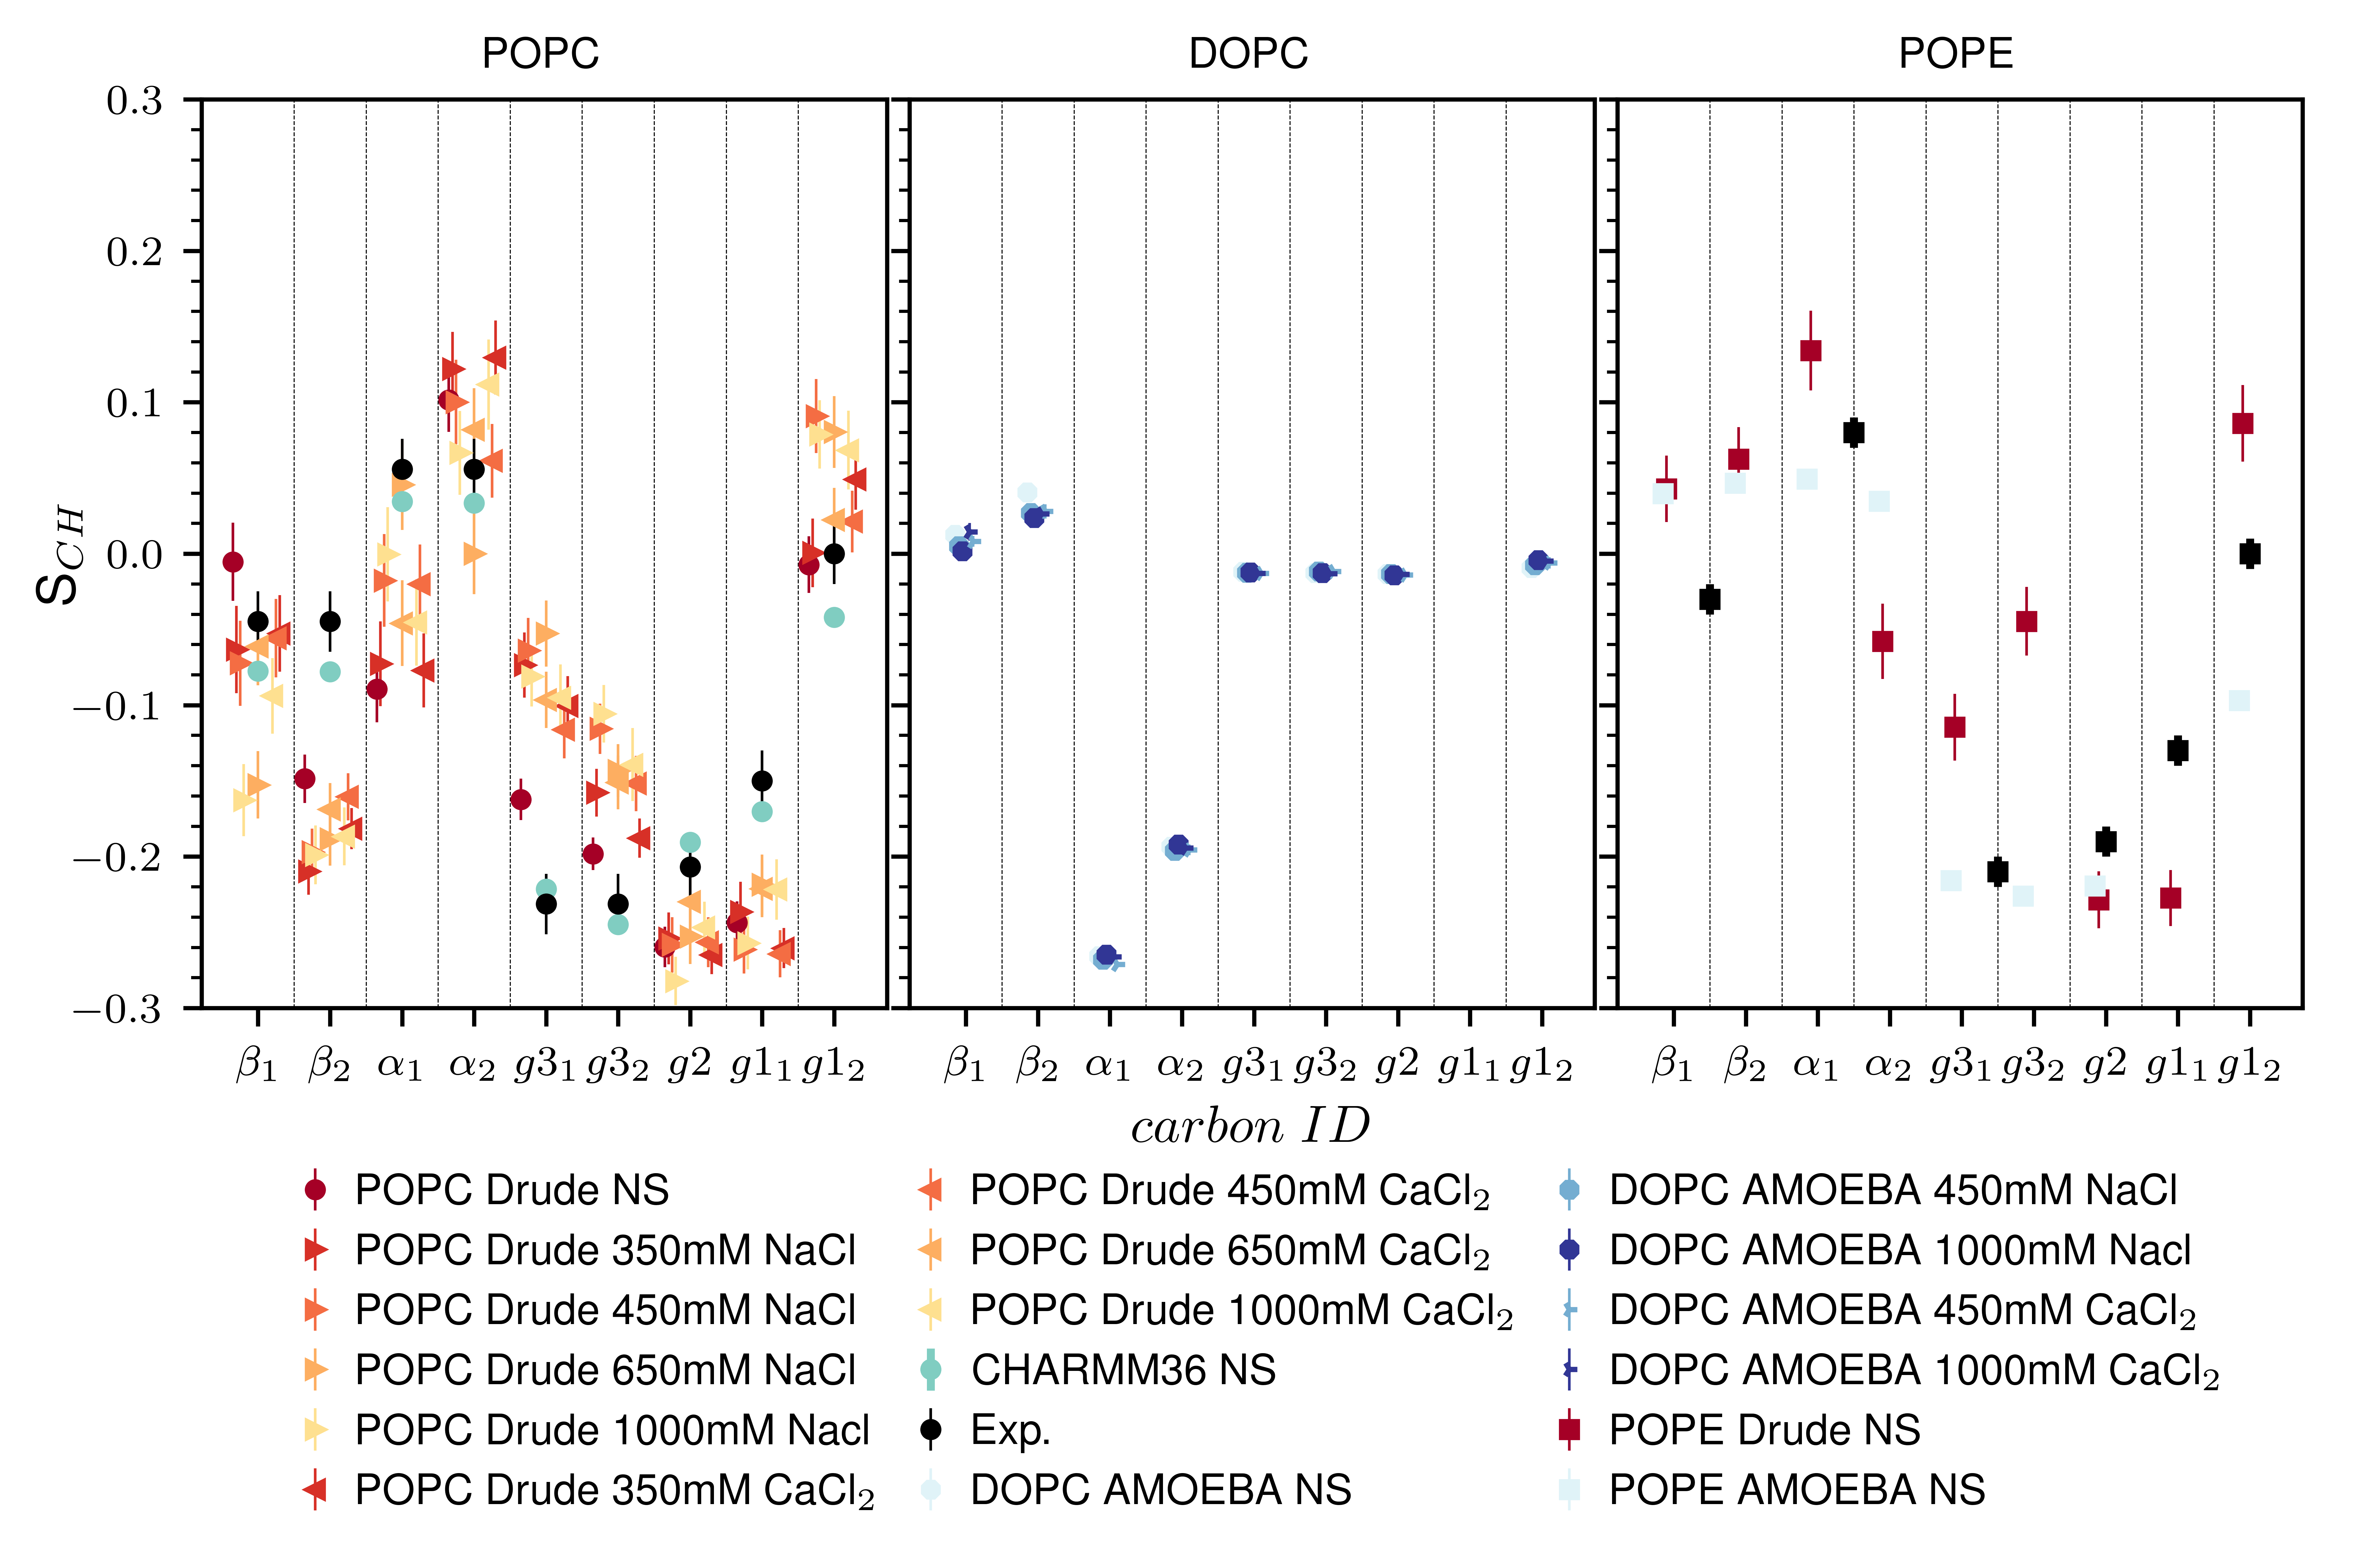
\includegraphics{Figures/order_parameters.png}
    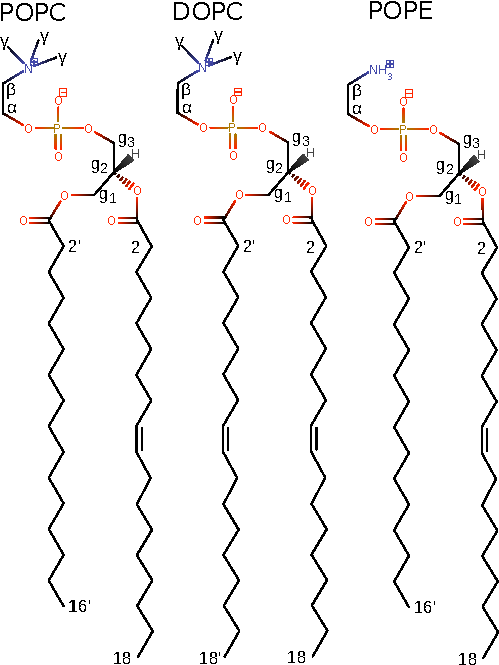
\includegraphics[width=0.4\textwidth]{Figures/molecules.pdf}
    \caption{Molecules and atom labelling used.}
    \label{fig:molecules}

\end{figure}


\begin{table}[]
    \centering
    \begin{tabular}{c c c c c c c}
        Lipid & Force field & $P^{\mathrm{headgroup}}$ & $P^{sn-1}$ & $P^{sn-2}$ & $FF_{q}$ & APL \\
        \hline
        POPC & OPLS3e       & 0.76 & 0.87 & 0.85 & 0.15 & 66.5\\
        POPC & CHARMM36     & 0.70 & 0.54 & 0.69 & 1.16 & 65.0\\
        POPC & CHARMM-Drude & 0.52 & 0.29 & 0.53 & 1.06 & 62.5\\
        POPC & CHARMM-Drude2023 & 0.63 & 0.60 & 0.57 & 0.96 & 64.5\\
        \hline
        POPE & GROMOS-CKP & 0.29 & 0.83 & 0.48 & 0.40 & 59.6\\
        POPE & CHARMM36   & 0.54 & 0.52 & 0.27 & 1.30 & 57.2 \\
        POPE & CHARMM-Drude & 0.06 & 0.53 & 0.27 & 0.80 & 56.6  \\
        POPE & CHARMM-Drude2023 & 0.28 & 0.59 & 0.54 & 0.00 & 61.4  \\
        POPE & AMOEBA & 0.21 & 0.10 & 0.23 & 3.80 & 66.9\\
        \hline
        DOPC & AMOEBA & 0.60 & 0.60 & 0.54 & - & 70.2\\
    \end{tabular}
    \caption{NMRlipids databank quality metrics~\cite{Databank} and area per lipids (APL) compared between the best simulations found from the NMRlipids databank (OPLS3e~\cite{roos19} for POPC and GROMOS-CKP~\cite{Chandrasekhar03,kukol09,piggot12} for POPE), simulations with CHARMM36 force field, and simulations with polarizable force fields. Order  parameter quality measures, $P^{\mathrm{headgroup}}$, $P^{sn-1}$, and $P^{sn-2}$, present the average probability of order parameters within a given segment to agree with experiments (larger probabilities mean higher quality). Form factor quality measure, $FF_{q}$, presents the difference in essential features between simulated and experimental form factors (smaller values indicate higher quality). Experimental estimations for areas per lipid are POPC: 64.3$\pm1$\AA$^{2}$\cite{kucerka2011}, DOPC: 67.5$\pm1$\AA$^{2}$\cite{kucerka2008}, and POPE: 56.7$\pm$3\AA$^{2}$\cite{Rickeard2020}.}
    \label{tab:my_label}
\end{table}



\begin{figure}[!p]
    \centering
    %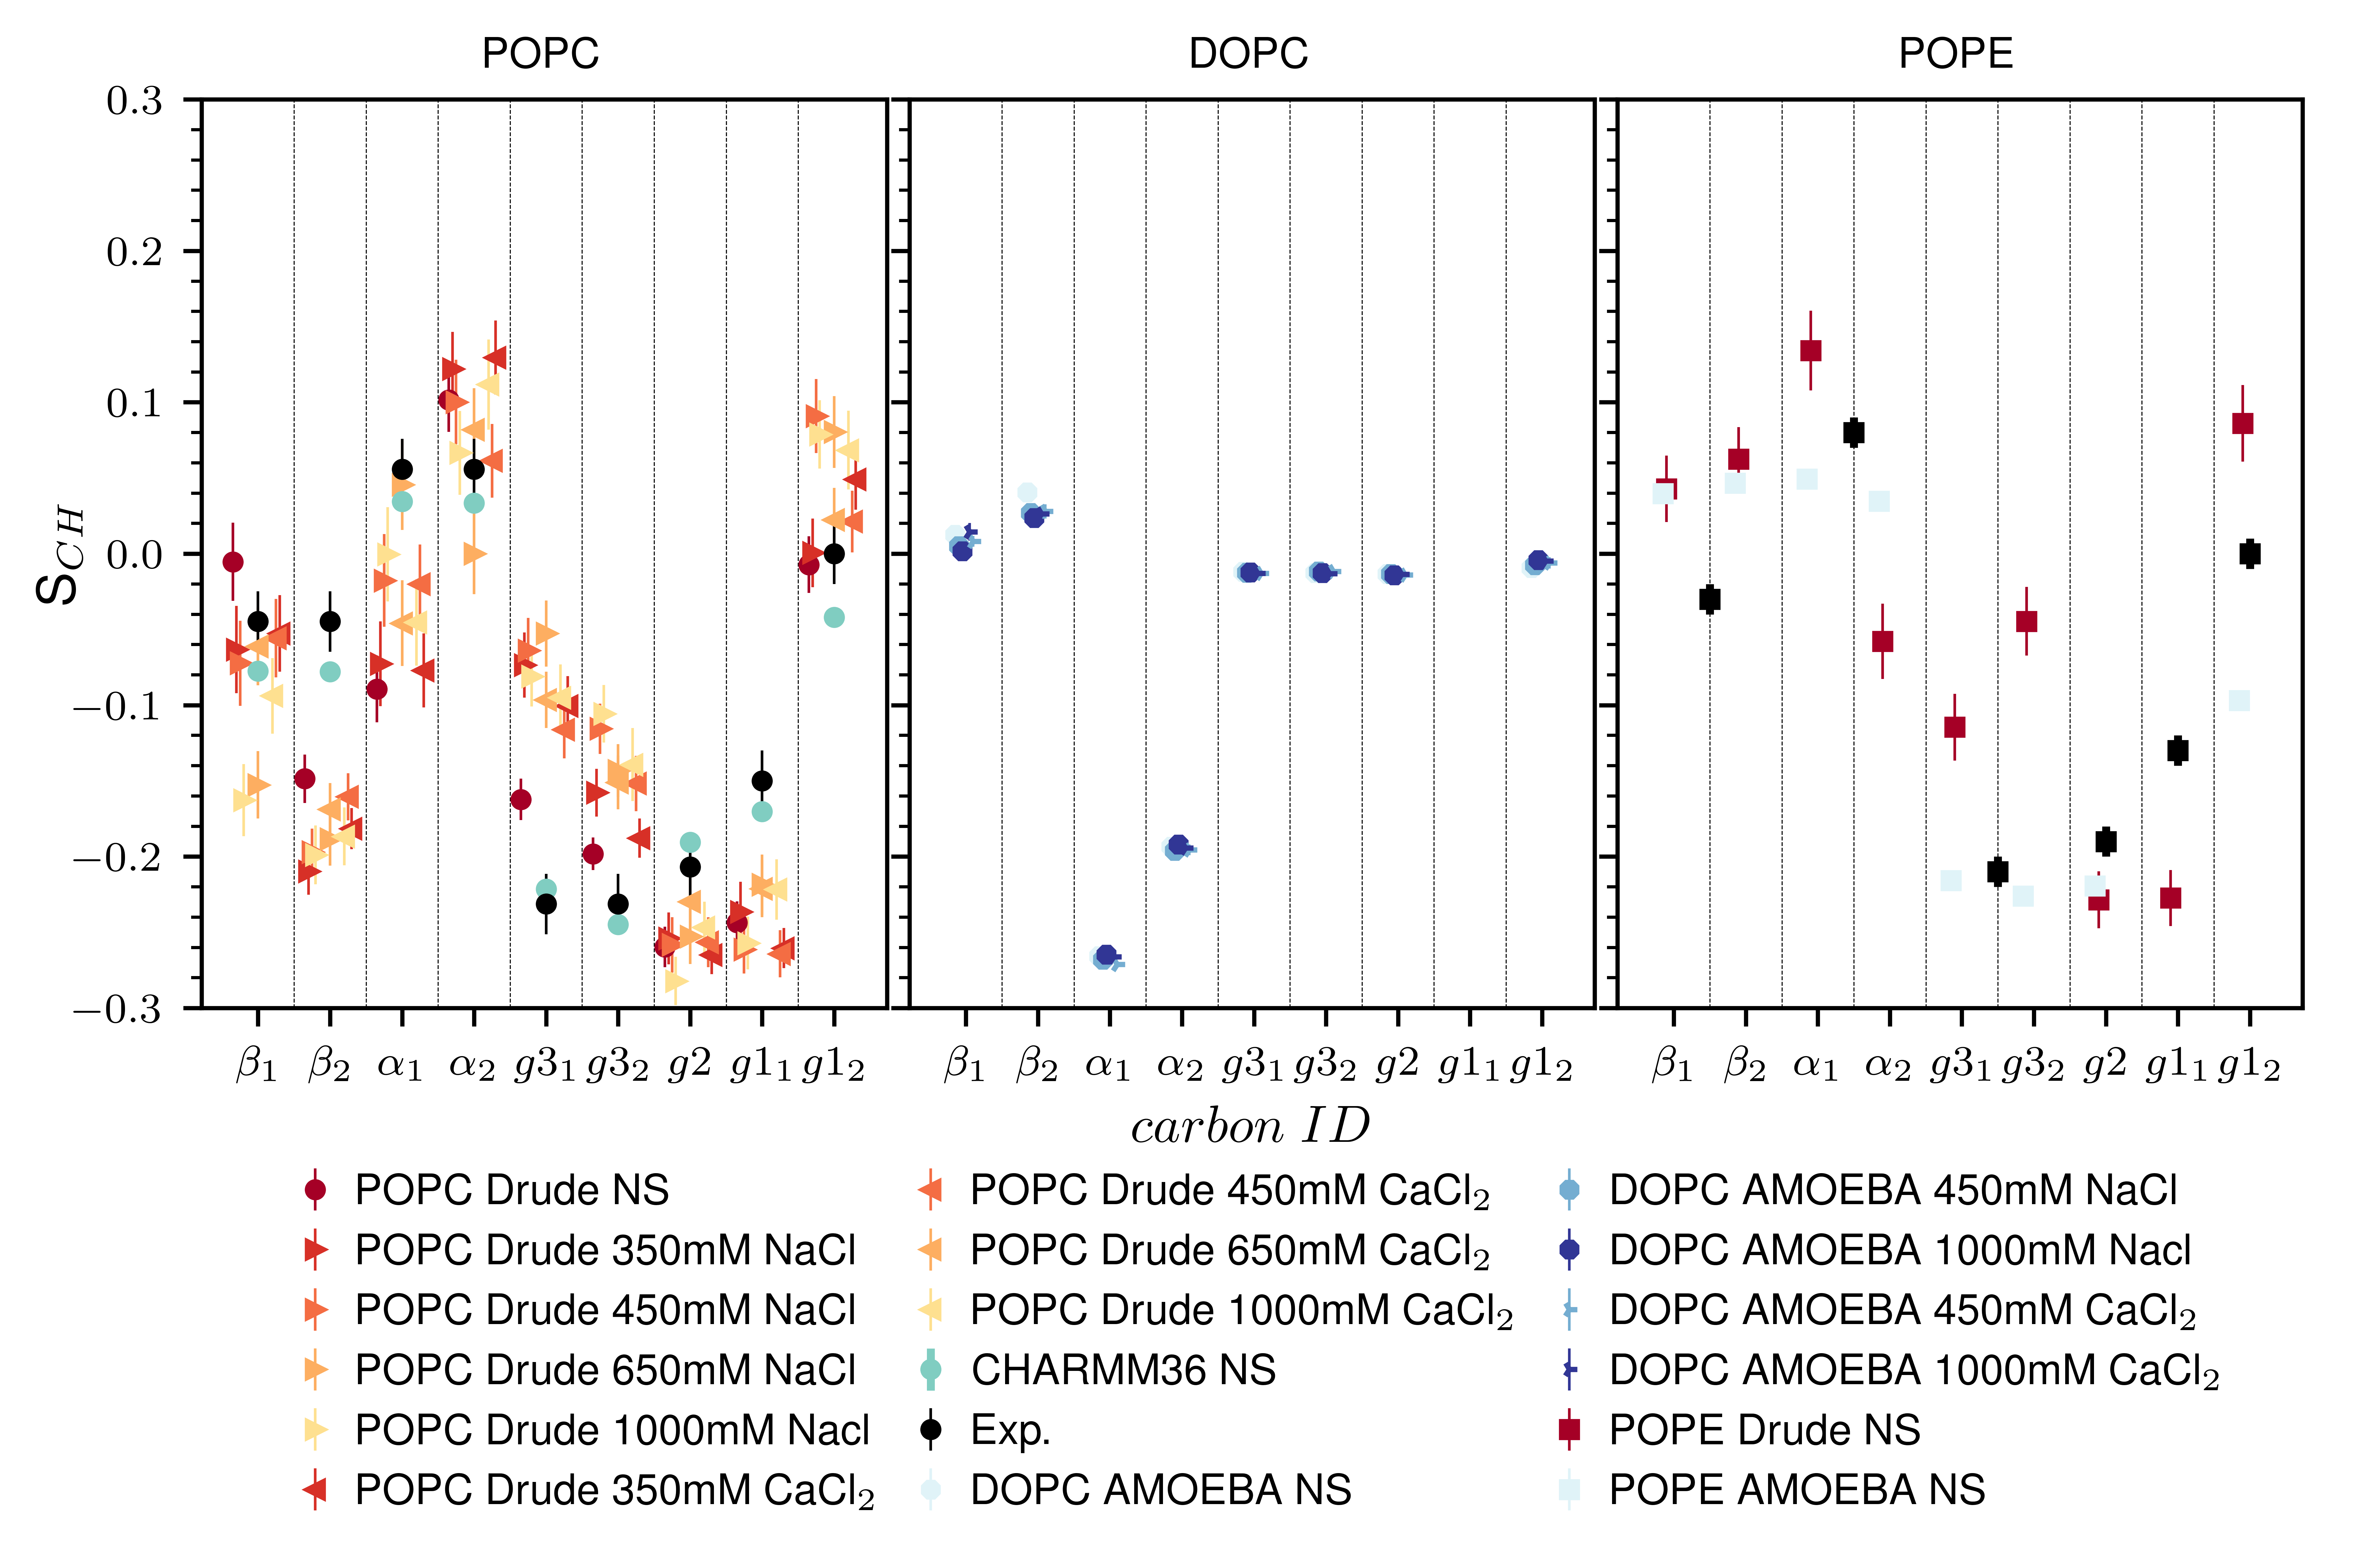
\includegraphics{Figures/order_parameters.png}
    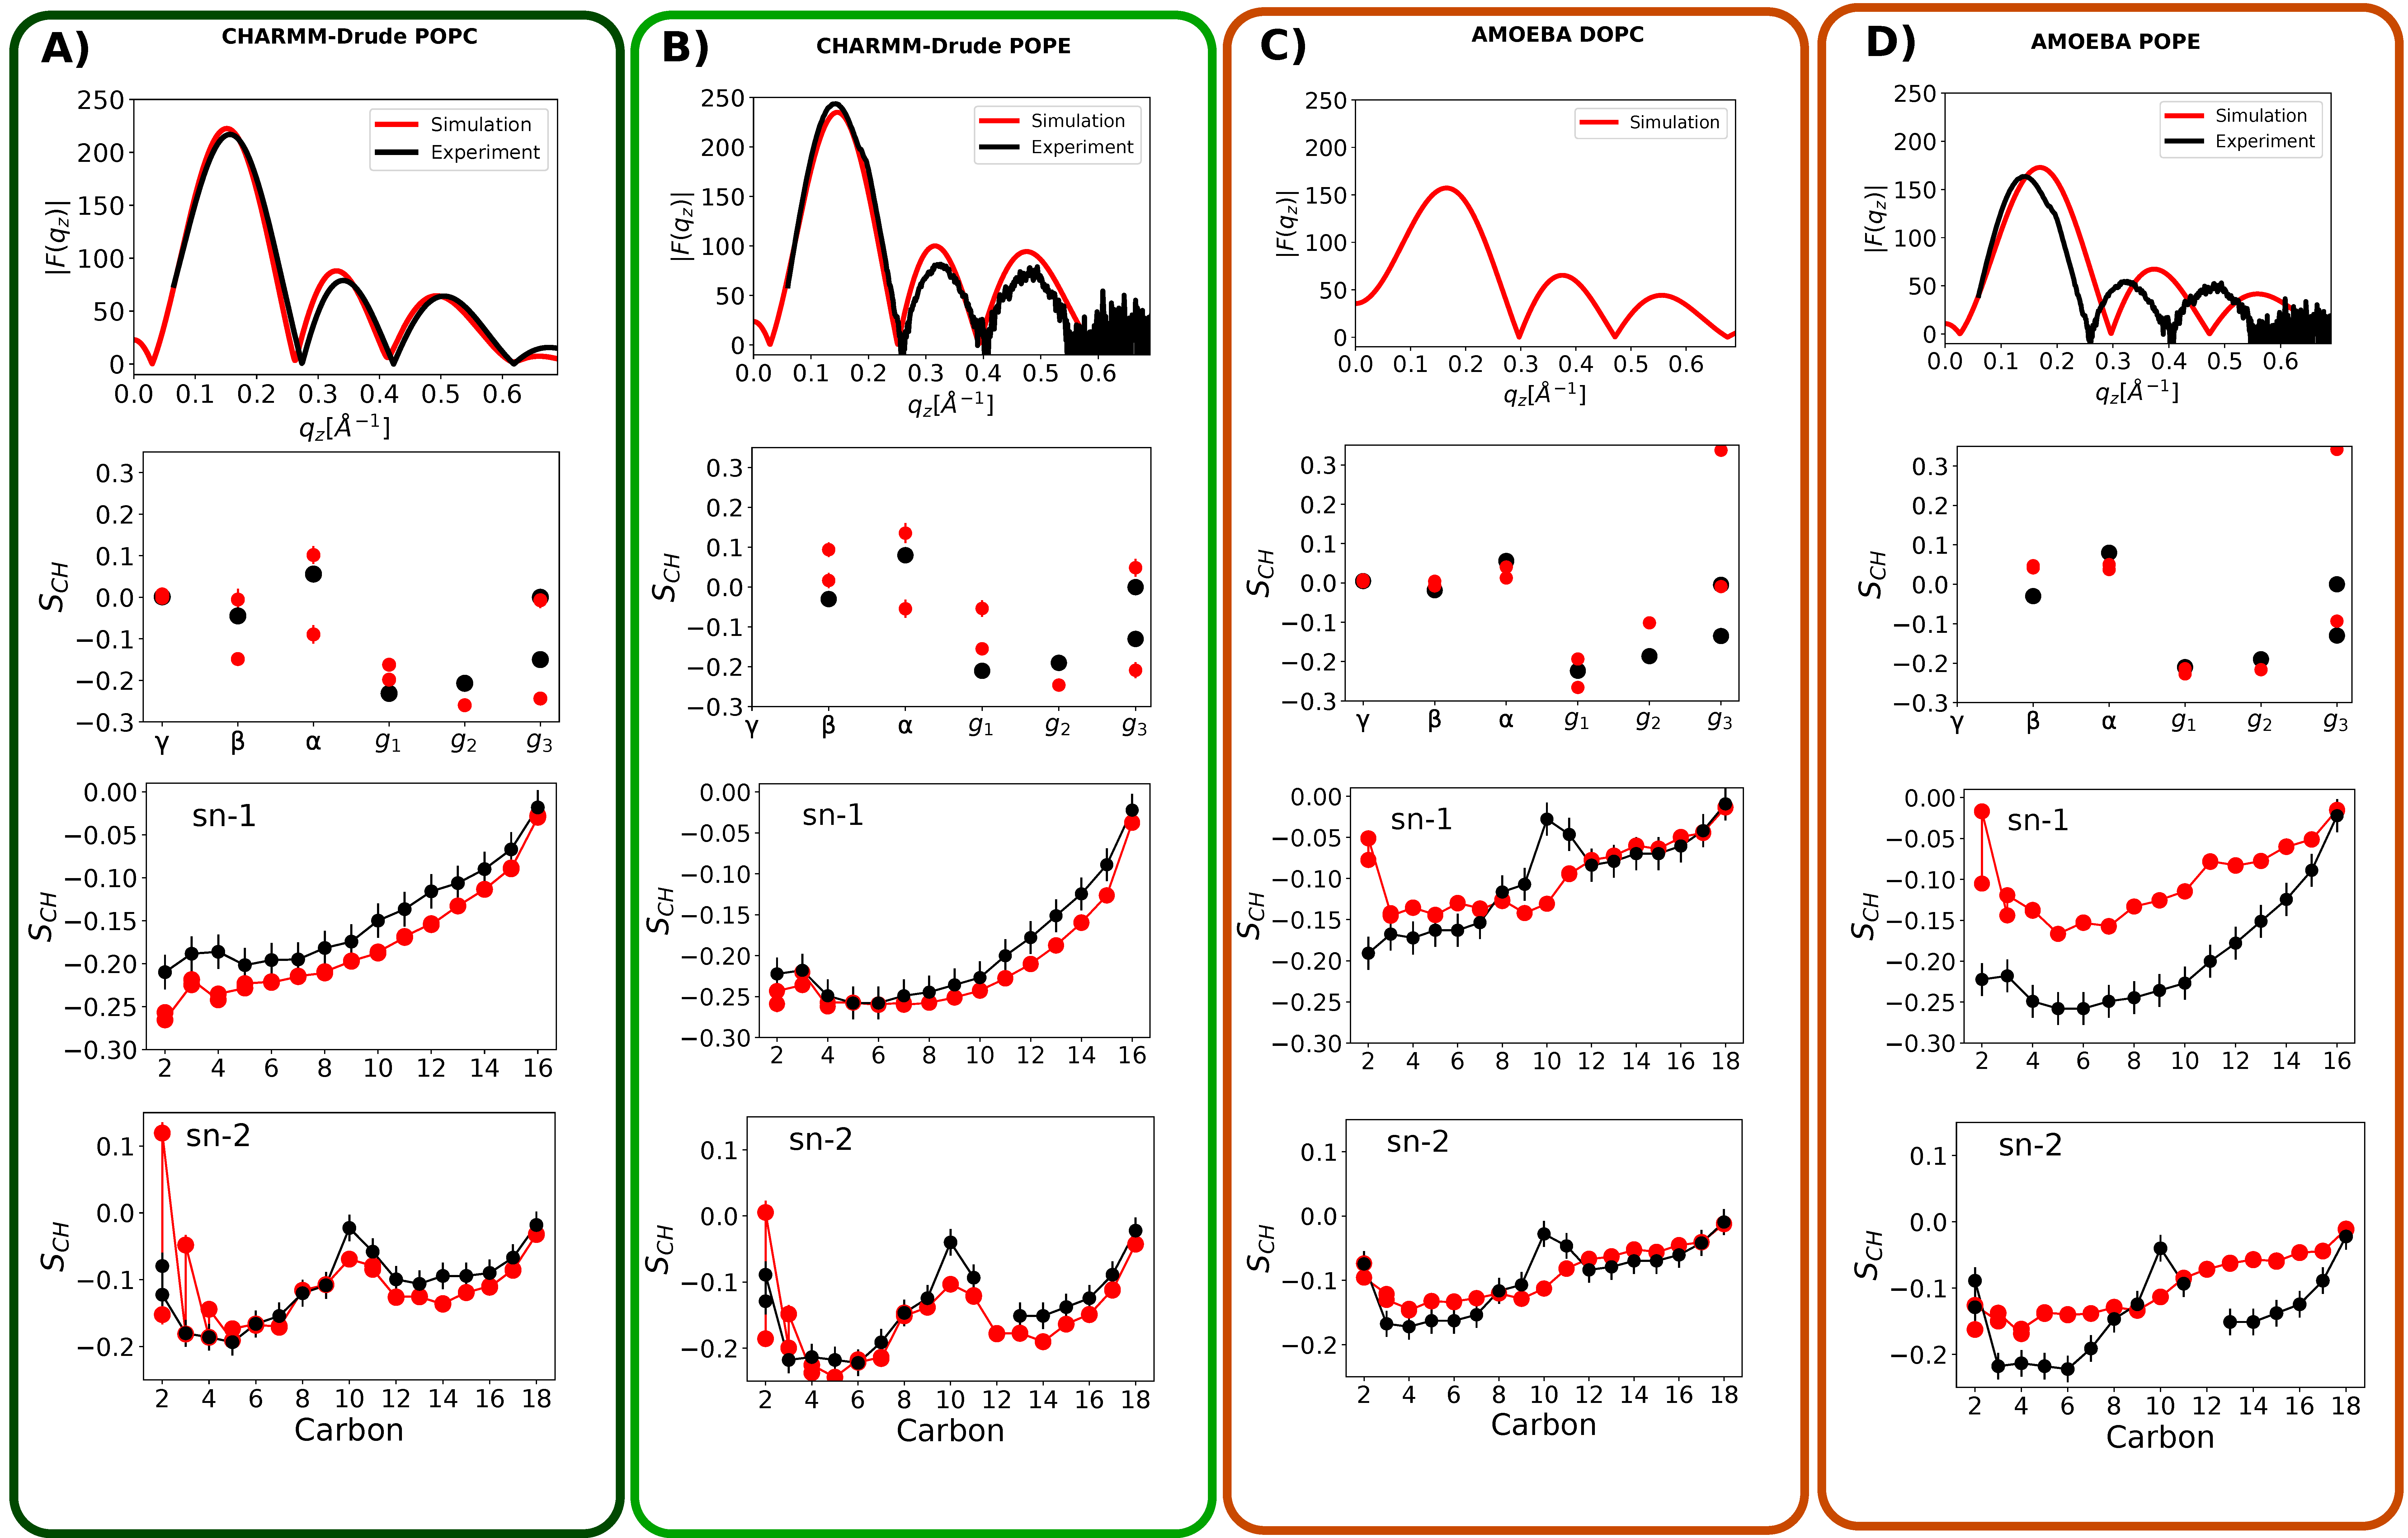
\includegraphics[width=0.8\textwidth]{Figures/quality.pdf}
    \caption{X-ray scattering form factors, and C-H bond order parameters for headgroup and glycerol backbone, and acyl chains (from top to bottom) compared between simulations and experiments using the NMRlipids databank. The atom labelling is as depicted in Fig.~\ref{fig:molecules}. Experimental data in this figure are originally reported in Refs.~\citenum{ferreira13,bacle21,Databank,NMRlipidsIII,kucerka2015}. For CHARMM-Drude2023 simulations we selected representative replicas among three available simulations, for example for differences between replicas for POPC see Fig.~\ref{fig:order_parameters_replicas}.}
    \label{fig:order_parameters}

\end{figure}

Direct comparisons between simulated and experimental data are visualized in Fig~\ref{fig:order_parameters} and the resulting quality metrics are shown in Table~\ref{tab:my_label}. Similarly to the non-polarizable CHARMM36 simulations, CHARMM-Drude simulation predicts slightly too packed membrane with excessively negative order parameters with respect to experiments and simulations with the highest quality in the NMRlipids databank (OPLS3e)~\cite{Databank}. However,
%consistently outperform the polarizable force fields with respect to the NMR measurables for all parts of the molecule (higher $P$-values). For older CHARMM-Drude force field, 
the quality of headgroup conformations in the CHARMM-Drude simulations is worse than in its non-polarizable counterpart. This is likely because headgroup and glycerol backbone parameters were optimized to reproduce absolute average values of the experimentally determined order parameters, instead of taking into account the order parameter forking (meaning measurably different order parameters for different C--H bonds at a single carbon atom) and order parameter sign~\cite{Antila2022}. A better description of the headgroup and glycerol backbone is provided by CHARMM36-Drude2023, yet its quality is still below that offered by the non-polarizable CHARMM36 parameters (see also discussion about conformational dynamics below). Also the quality of membrane packing and acyl chain order are improved in CHARMM36-Drude2023 compared to the earlier version but again, it did not perform at a quality comparable to that of the best available simulations.
%also provides better description of the carbon tails. 
%In fact, for POPE sn-2 tail the CHARMM-Drude2023 gives the best description of the models investigated here.  

 AMOEBA simulations capture the headgroup and glycerol backbone order parameters reasonably well with the exception of g$_1$,
%ll for both DOPC and POPE but vastly overestimates one of the g$_3$ values, resulting in 
where forking of order parameters is unacceptably large. However, experimentally observed low order parameters at double bond region in both DOPC acyl chains and {\it sn}-2 chain of POPE are not captured. These low order parameters signal an important mechanism through which acyl chain double bonds affect membrane properties~\cite{ollila07} and are well reproduced in all state-of-the art MD simulation parameters~\cite{ollila16}. Furthermore, AMOEBA parameters substantially overestimate the area per lipid in POPE simulations, leading to too disordered acyl chains. Similar issues are evident also in membrane data presented in the recent publication for the AMOEBA cholesterol model~\cite{Li23chol}.
%also clearly struggles to depict the tail conformations, in particular in the double bond region of DOPC (Fig.~\ref{fig:order_parameters}). 
%parameters do not capture the  
%In the tail regions, the CHARMM-Drude2023 appears to be the best out of the polarizable models. 
 

The unsatisfactory description of the lipid tail region and the area per lipid is further reflected in the inability of AMOEBA to capture the SAXS curves. Thus, we can conclude that our simulations with the AMOEBA parameters did not reproduce essential
membrane properties. The higher $FFq$ values (Table~\ref{tab:my_label}) of the polarizable force fields in general indicate that they are not able confer consistency with the SAXS data as well as the best non-polarizable force fields (OPLS3e). That said, CHARMM-Drude2023 is on par with or better than its non-polarizable counterpart CHARMM36 and the best out of all the models here in capturing the POPE SAXS data, benefiting from the improvements made in the description of acyl chains.




\subsection{Evaluation of conformational dynamics of lipids}
C-H bond order parameters are sensitive to the conformational ensemble but the correspondence is not unique. Instead, they essentially describe the average of the distributions and do not contain information of the dynamics of the conformational sampling. Therefore, a simulation that reproduces the order parameters has an ensemble that is only potentially correct, and even the correct ensemble may not have the experimentally observed dynamics. To further elucidate this aspect in the case of polarizable force fields, we compared NMR $^{13}$C spin relaxation $R_{1}$ rates and C-H bond effective correlation times $\tau_{\mathrm{eff}}$ with experiments~\cite{ferreira15} and best non-polarizable simulations from our previous study~\cite{Antila2021} for simulations with PC headgroups and the glycerol backbone in Fig.~\ref{fig:correlation_times}. This focus was chosen based on the availability of both experimental data and polarizable simulations. $R_{1}$ rates measured with typical magnetic field strengths are sensitive to rotational dynamics of C-H bonds with the timescales around $\sim$0.1-1~ns, while effective correlation times respond to a larger range of dynamical processes up to $\sim$1000~ns~\cite{ferreira15}. The effective correlation time can be interpreted as an average measure for how fast molecular conformations sample the phase space that leads to the average order parameters.

The effective correlation times in CHARMM-Drude2017 and CHARMM-Drude2023 simulations are approximately two  and one orders of magnitude slower, respectively, than the values suggested by experiments and best available simulations (Fig.~\ref{fig:correlation_times}). This indicates that not only are the simulations with this polarizable force field computationally costlier for equivalent lengths of trajectory, but one would also have to simulate longer to obtain converged results. The non-polarizable counterpart of the Drude models, CHARMM36, exhibits much more realistic, faster effective correlation times. Also the dynamics in the fast range ($R_{1}$ rates), are on average slightly more realistic in the non-polarizable CHARMM36 compared to both of the polarizable counterparts. Interestingly, CHARMM-Drude models have been reported to have slower water hydrogen bonding dynamics around amino acids compared to their non-polarizable counterpart,~\cite{Ngo2019} which might align with an overall slower dynamics of the model in addition to enhanced water binding. 

In contrast to the Drude-based models investigated here, the $R_1$ spin relaxation times and effective correlation times from DOPC simulations with AMOEBA force field are close to experimental data from POPC and on par with the best non-polarizable models (Slipids and CHARMM36). The small difference in acyl chain composition (DOPC vs. POPC) is not expected to strongly affect headgroup dynamics due to effective decoupling between hydrophilic and hydrophobic membrane regions~\cite{Antila2022rot, Klauda08}.
%appears to be faulty in the fast range ($R_{1}$ rates) and, furthermore, $\tau_{\mathrm{eff}}$ values reveal vastly too slow overall dynamics. The updated CHARMM-Drude2023 does not significantly improve the dynamics at the fast range investigated here. The effective correlation times of the newer Drude model are improved but still an order of magnitude too slow. This indicates that not only are the simulations with this polarizable force field computationally costly but one would have to simulate longer to obtain converged results. The non-polarizable counterpart of the Drude model, CHARMM36, exhibits much more realistic, faster effective correlation times. 
%Interestingly, it has also been observed that CHARMM-Drude models have slower dynamic of water hydrogen bonding around amino acids compared to their non-polarizable counterpart~\cite{Ngo2019} which might align with an overall slower dynamics of the model in addition to enhanced water binding. 
%Note that the experimental data here is from POPC. However, chemically identical the headgroup region the dynamics is assumed to be practically identical in DOPC, due to the decoupling of the dynamics between the headgroup and the glycerol regions~\cite{Antila2022rot, Klauda08}.

%We include the same measurables calculated from non-polarizable CHARMM36 and SLipids force fields---the best MD force fields regarding the dynamics~\cite{Antila2021}---as a point of comparison. 

\begin{figure}[!hbt]
	\centering
	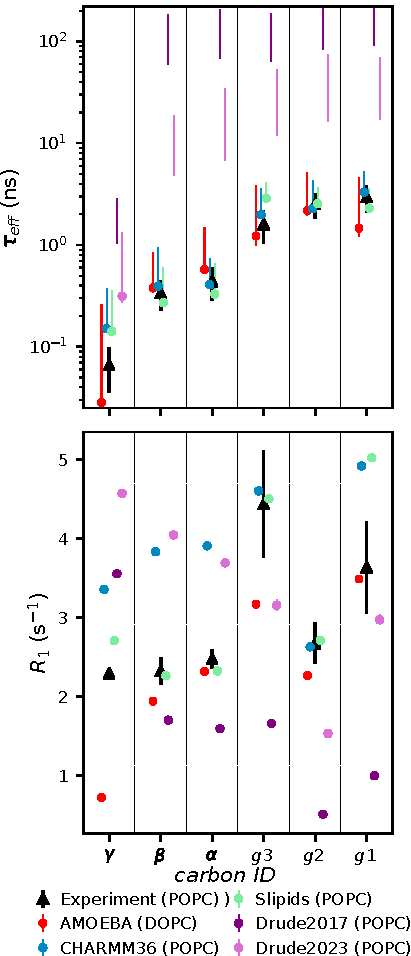
\includegraphics{Figures/both_inkscp.pdf}
	\caption{Effective correlation times (top) and R$_1$ rates (bottom) for the polarizable models and best performing non-polarizable force fields. Note, top panel axis is logarithmic to visualize the slow Drude dynamics. Experimental values are obtained from Ref.~\citenum{Antila2022rot}. All simulations used here were salt free.}
	\label{fig:correlation_times}
\end{figure}


\subsection{Cation binding to membranes in polarizable simulations}

Given the abundance of cations in biological systems, accurately capturing their interactions with membranes has the uttermost importance in MD simulations. A wealth of  experimental evidence shows that monovalent ions (except for lithium) exhibit very weak binding affinity of PC lipid bilayers, while multivalent ions like calcium bind more strongly~\cite{Catte2016}. However, simulations with non-polarizable force fields without any additional corrections systematically overestimate cation binding to lipid bilayers~\cite{Catte2016}. Implicit inclusion of electronic continuum correction (ECC) to both ion and lipid parameters can substantially improve the situation~\cite{Melcr:2018a,melcr2019improved,bacle21}, suggesting that electronic polarizability plays an important role in ion binding to membranes, which might further lead one to expect that that simulations with polarizable force fields will perform better in this aspect and more accurately describe ion binding to membranes.
%Finally, we address the premise that adding polarizability to force fields improves the depiction of ion binding to biomembranes in simulations. 
To test this notion, we evaluated ion binding to membranes against the experimental NMR data using the "lipid electrometer," which involves quantifing the amount of ion binding to the membrane by monitoring the change in lipid headgroup order parameters in response to increasing salt concentration~\cite{Catte2016}. Changes in these order parameters induced by increasing NaCl and CaCl$_2$ are shown in Fig.~\ref{fig:popc_order_parameter_change} for simulations and experiments, whereas Fig.~\ref{fig:ion_density_profiles} shows the density profiles of ions with respect to the bilayer normal. Results from AMBER-based ECC-lipid model are shown for the reference that gives a good agreement with experiments for cation binding. We also show data from the non-polarizable CHARMM36 where NBFIX correction for the ion models was specifically developed to address overbinding~\cite{Venable2013,Han2018}.

\begin{figure}[!hbt]
	\centering
	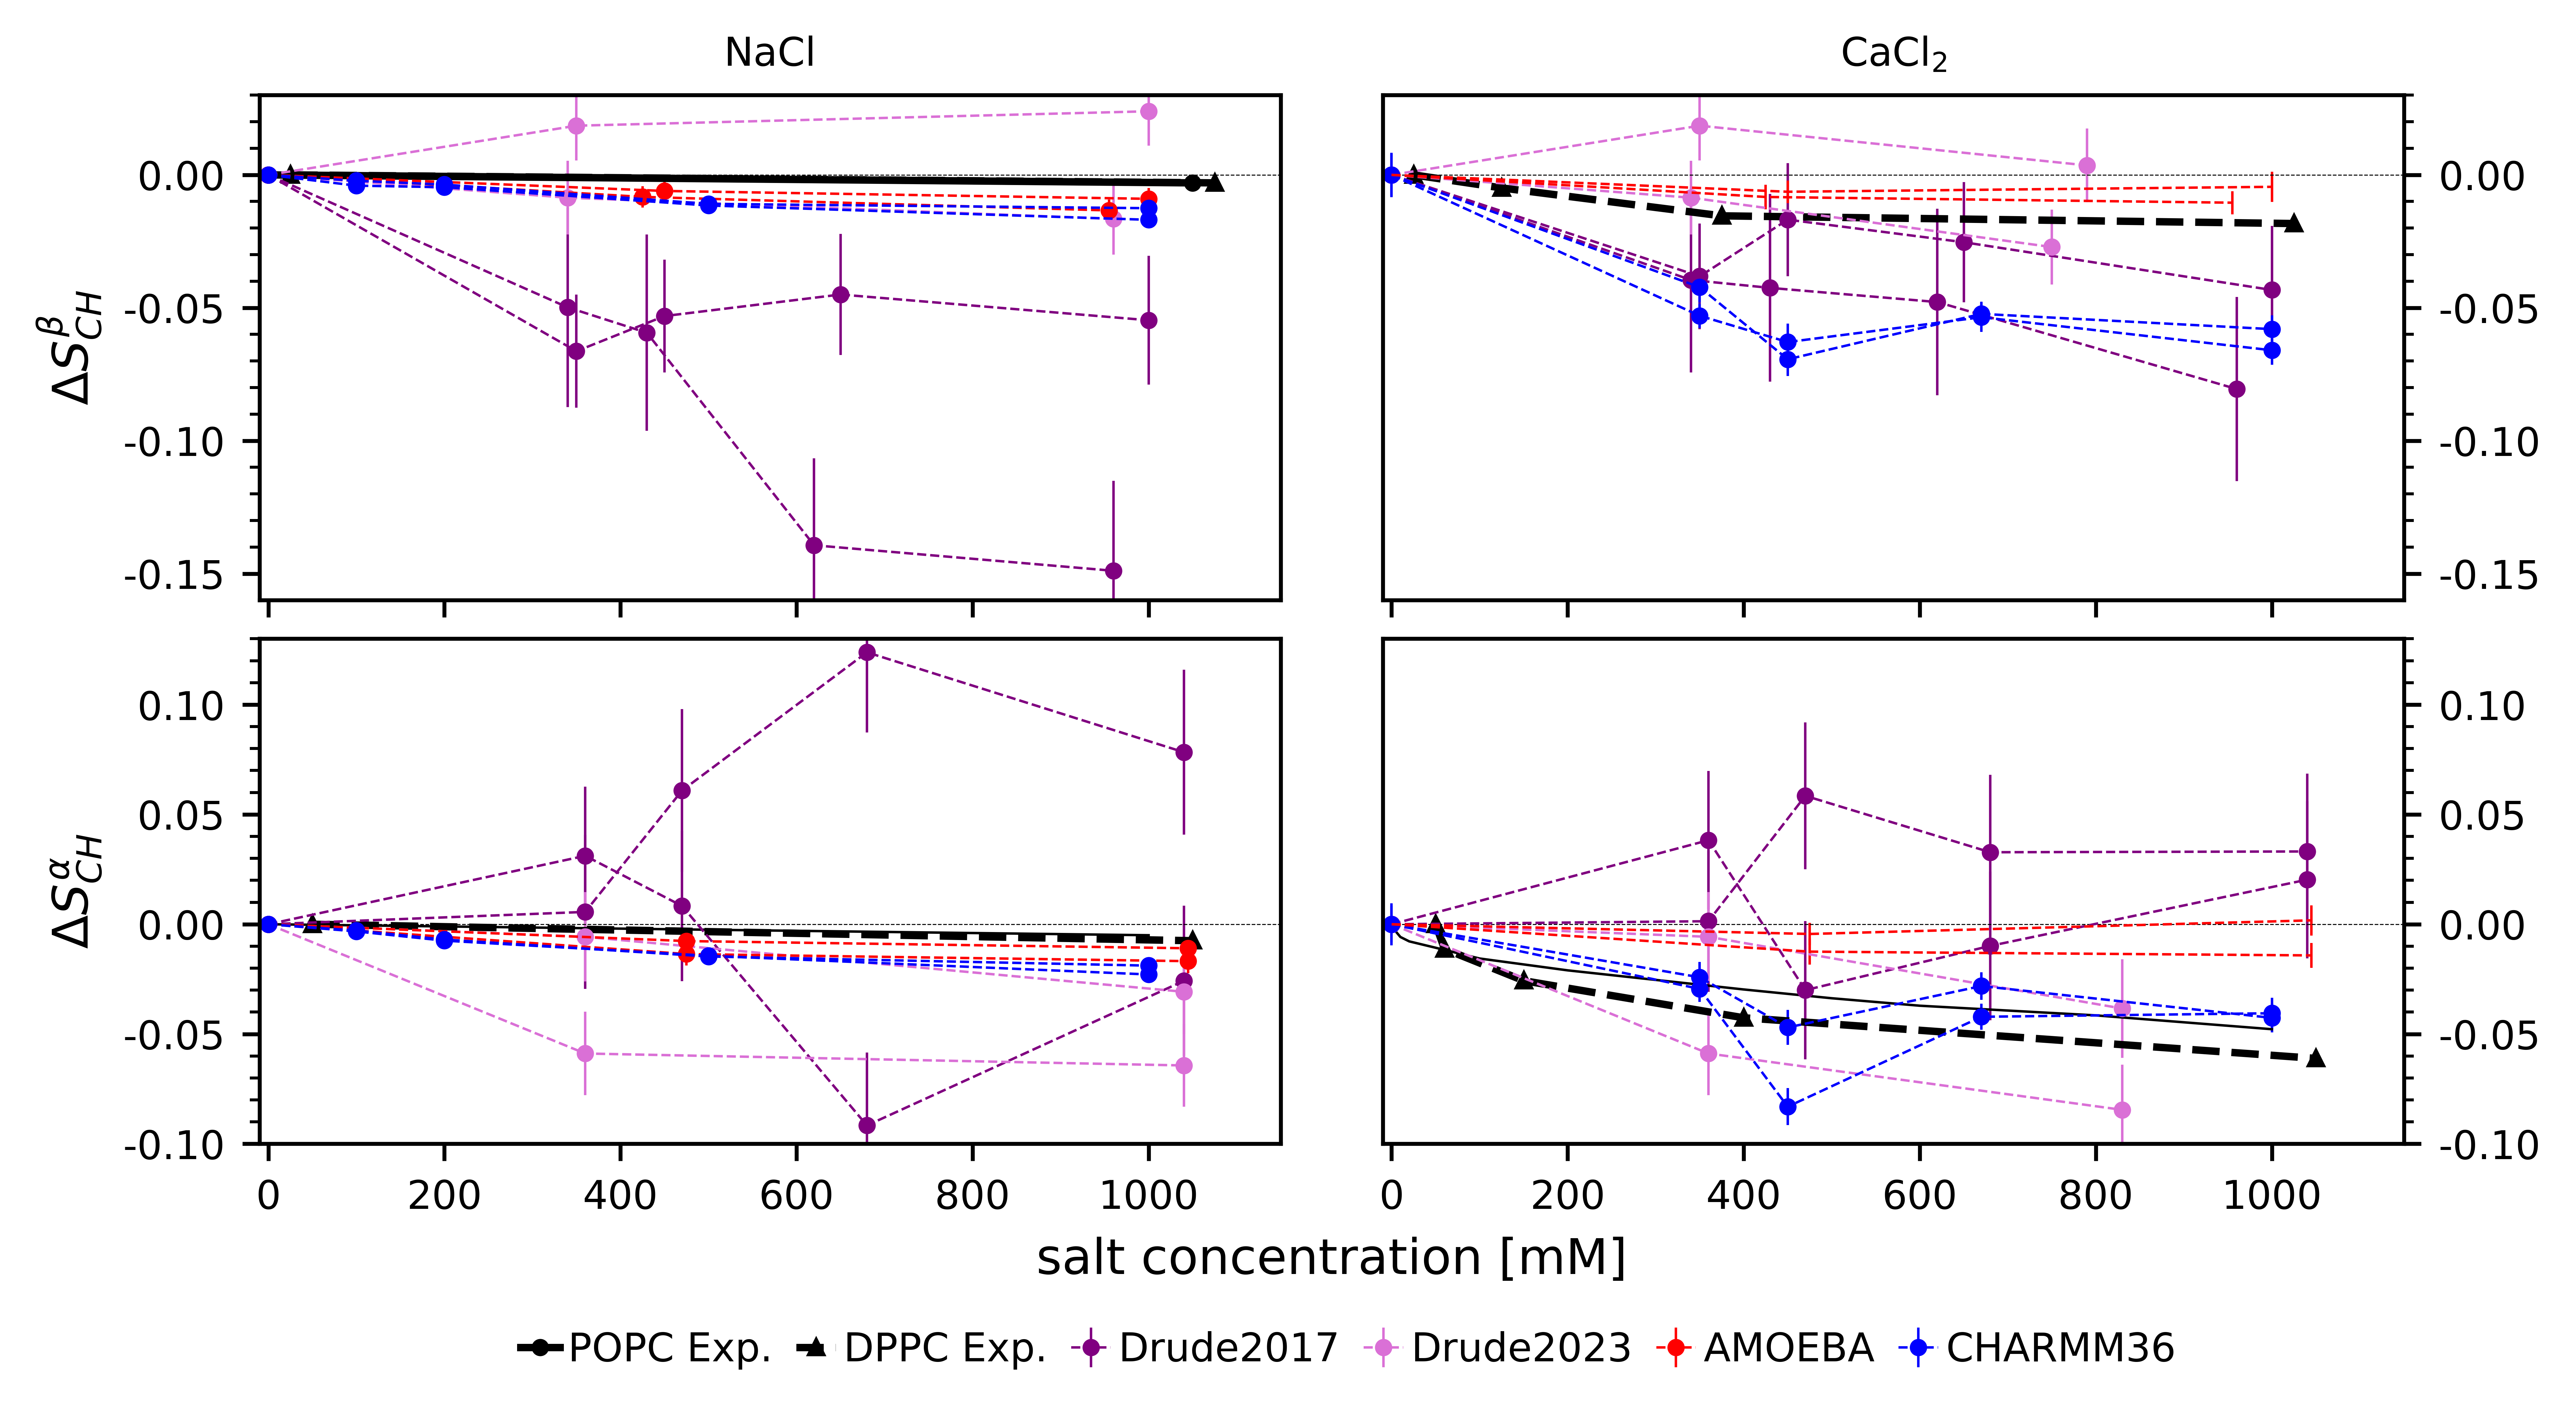
\includegraphics{Figures/order_parameter_change.png}
	\caption{The change in the lipid head group order parameters $\beta$ (top row) $\alpha$ (bottom row) upon increasing ion concentration with respect to the simulations without salt. CHARMM36 and ECC data is reproduced using the Zenodo repositories Ref.~\cite{ollila_2015_32496, ollila_2015_32497, ollila_2015_32498, nencini_ricky_2019_3434396} and Ref.~\cite{melcr_josef_2017_3335503}, respectively.}
	\label{fig:popc_order_parameter_change}
\end{figure}

\begin{figure}[!hbt]
    \centering
    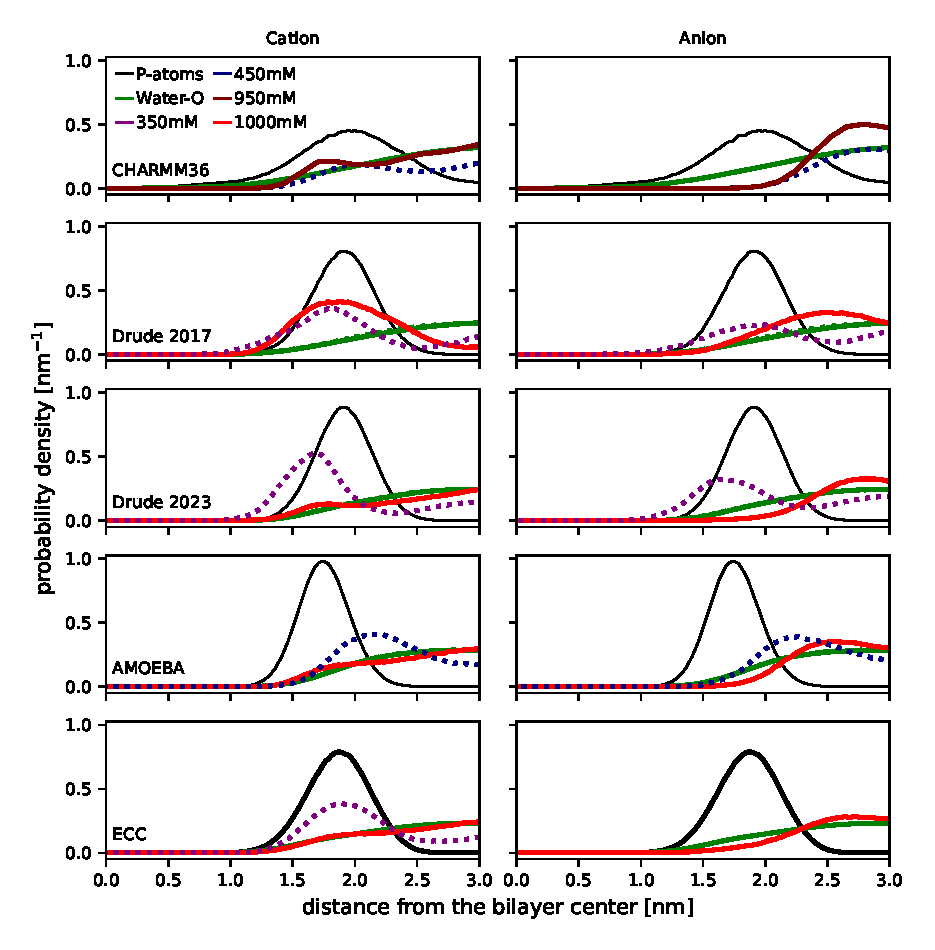
\includegraphics{Figures/ion_density_profiles_with_chloride.eps}
    \caption{Density profiles along the membrane normal for the CHARMM36 (first row)~\cite{Catte2016}, Drude 2017 and 2023 POPC (second and third rows), AMOEBA DOPC (fourth row), and electronic continuum correction (ECC, last row)~\cite{Melcr:2018a}. Solid and dashed lines are for the systems with the NaCl and CaCl$_{2}$, respectively. Please note that only 350~mM and 450~mM CaCl$_{2}$ concentrations are shown for the Drude and AMOEBA force fields, respectively, while 1000~mM NaCl concentration is shown for all force fields. CHARMM36 NaCl simulations are at 950~mM. CHARMM36 data is reproduced using the Zenodo repositories Ref.~\cite{ollila_2015_32496, ollila_2015_32497, ollila_2015_32498, nencini_ricky_2019_3434396}}
    \label{fig:ion_density_profiles}
\end{figure}

The CHARMM-Drude2017 predicts similar calcium ion density profile to ECC-lipids, in good agreement with experiments. However, the sodium binding is equally strong in these simulations in contrast with the experimental evidence~\cite{Catte2016}. 
%, evidenced both by large change in the order parameters and the ion density profiles. Based on the change in the order parameters, the sodium binding is even stronger than the divalent calcium binding. In strong contrast, experimentally one sees no sodium binding and some binding of calcium ions. 
Excessive sodium binding in the CHARMM-Drude model has been observed before for systems containing peptides or amino acids~\cite{Ngo2019, Kav2022} and deep-eutectic solvents~\cite{shayestehpour2022ion}. Excessive calcium interactions, in line with what we observe here for the lipids, have also been reported~\cite{Tan2022}. Furthermore, the response of headgroup order parameters to the bound ions is not in qualitative agreement with experiments for CHARMM-Drude2017 simulations according to Fig.~\ref{fig:popc_order_parameter_change}. Particularly, increasing $\alpha$ carbon order parameters and forking upon ion binding are not observed in experiments. This is in contrast with the results from previous bechmarking of non-polarizable simulations~\cite{Catte2016}, where experimentally observed decrease of order parameters to more negative values upon ion binding were observed in all simulations, even though the binding affinity was often inaccurately predicted. This qualitative discrepancy in CHARMM-Drude2017 simulations most likely results from incorrect lipid headgroup conformational ensemble (see previous sections), which leads to inaccuracies in the structural response of the ensemble to ion binding. 

In simulations with CHARMM-Drude2023 parameters, sodium ion binding is in line with ECC-lipid simulations when comparing density profiles,
%force field: the change of the order parameters is diminished to be more in line with experiments and only the some accumulation of sodium ions near the phosphate oxygen is seen in the ion distributions. 
%However, this the ion layering is most prominently present in the original CHARMM36 force field, for for sodium and calcium ions. 
but addition of sodium or calcium ions seems to induce forking of order parameters in contrast to experiments. 
%at the $\beta$ carbon in particular. 
This might indicate inaccurate structural response to ion binding, but poor convergence of the simulations owing to the slow conformational dynamics detected above cannot be ruled out in this case or in the case of the older 2017 version.
%, which would also not be fully reflected in the calculation of error estimates for the order parameters. 
Based on density profiles, calcium binding in CHARMM-Drude2023 simulations is in line with the ECC-lipid model, although binding affinity is slightly larger, 
%also appears to be better represented in the updated model. The 
ions penetrate 
%reveal that binding of calcium has moved 
deeper into the bilayer, and there is a stronger formation of ionic double layer by subsequent attraction of chloride into the bilayer.  
In the non-polarizable counterpart, CHARMM36 model with the NBFIX correction, sodium biding is similar to the polarizable models outside small accumulation peak in the phosphate region, and stronger subsequent accumulation of anions outside the phosphate region. The structural response well in line with the experiments. The divalent cation biding for CHARMM36 is weakest of all models with binding depth, and following anion binding, quite similar the ECC. However, the structural response of the $\alpha$ carbons is weaker than in ECC and experiments. Contrasting the CHARMM36 with the CHARMM-Drude models and the ECC model results suggests that so far correcting the ion biding by scaling the Lennard-Jones parameters (NBFIX) of the non-polarizable models has resulted in slightly more realistic ion binding than introducing explicit polarizability to the model. 
%As opposed to the CHARMM36-Drude model, the order parameters of the AMOEBA model are almost completely unaffected by the ion addition, both for NaCl and CaCl$_{2}$. The ion density profiles confirm that very little ions penetrate the membrane region where the lipid phosphates reside. While this is in line with experiments regarding sodium ions, there should be some binding of calcium ions to the membrane. 
In AMOEBA simulations, sodium binds weakly and does not affect order parameters, consistent with experiments and ECC-lipid simulations. However, order parameters also do not change upon calcium binding contrasting the experiments. This can be explained by the binding position of calcium, which is outside phosphate density peak in AMOEBA simulations. In simulations where calcium penetrates to phosphate region or deeper in similar amounts, it reorients the headgroup dipole, giving rise to changes in order parameters~\cite{Catte2016}. 


%Again, the change in the order parameters indicate the non-polarizable CHARMM36 depicts sodium binding the best out of the models compared here, being slightly more realistic than its most recent polarizable counterpart, CHARMM-Drude2023. Regarding calcium binding, CHARMM36 captures the $\Delta^{\alpha}_{CH}$ about as well as the CHARMM-Drude2023, but the change in the $\beta$ carbon is better represented in the CHARMM-Drude2023 and AMOEBA models. This suggest that some accuracy might have been gained in modelling the divalent ion binding with polarizable models but the advantage is not clear. No force field, polarizable or non-polarizable, is able to model both monovalent and divalent ion binding flawlessly. This is of note, as polarizable force fields are often assumed superior and concequently a popupar choice in modelling, eg, ion channels~\cite{sun2017 jing2019polarizable, klesse2020induced}
%\begin{figure}[!hbt]
%	\centering
%	\includegraphics{dihedral_distributions_for_all.png}
%	\caption{The distributions of the torsion angles for the head group atoms}
%	\label{fig:dihedral}
%        \todo{SAMULI: I am not sure if we need this figure at all.
%          Or were you planning to discuss why order parameter response to ions is qualitatively incorrect in Drude PC?
%          If yes, then maybe remove POPE from this figure.
%        }
%\end{figure}

%\clearpage

%\clearpage

In conclusion, incorporating explicit polarizability as done in CHARMM-Drude or AMOEBA force fields does not necessarily lead to improved description of cation binding to phospolipid membranes. However, it is difficult to isolate the explicit influence of polarizability per se on ion binding based on the results presented here. What is clear, however, is that the headgroup conformational ensemble, which presumably plays a role in ion binding, is poorly described by the CHARMM-Drude parameters. In addition, the AMOEBA parameters struggle to capture the basic membrane properties that are reproduced by all current state-of-the-art MD simulation models.


\subsection{Discussion}

\textcolor{red}{For the ion binding discussion: drude calcium overbinds to proteins. this is known here https://pubs.acs.org/doi/full/10.1021/acsphyschemau.1c00039
drude sodium overbinds to proteins, as shown here https://pubs.rsc.org/en/content/articlepdf/2022/ra/d2ra01478e and https://onlinelibrary.wiley.com/doi/abs/10.1002/adts.201800106. Venable also cautioned us against using any ion parameters with the drude force fields. This is important as 1- polarizable force fields are supposed to be better for ion parameters and 2- they are generally used to study the ion channels.}

\subsection{Conclusions}
We have rigorously compared simulation output of model lipid bilayers using polarizable lipid force fields with high-resolution experimental data as well as results from best-performing non-polarizable force fields. From this, it is evident that current polarizable force fields for lipids fall short in important aspects. In most cases, the best non-polarizable models exhibits superior performance and accuracy in the categories investigated in this study.

Evaluation order parameters and scattering form factors reveals that the AMOEBA force field has difficulties in producing membranes with reasonable physical properties. In contrast, the CHARMM-Drude2023 model has improved performance in this regard, notably surpassing its predecessor, CHARMM-Drude2017. Nevertheless, top-performing non-polarizable models generally reproduce experimental conformations (order parameters) better, although not perfectly so.

In regard to conformational dynamics, the AMOEBA force field produces results, specifically in the headgroup region of PC lipids, that are either on par with or better than the best non-polarizable force fields. However, the CHARMM-Drude models exhibit an extremely slow dynamics, which can lead to deficient sampling and a substantial increase in required simulation time when using this model.


In general, the ECC model gives the most accurate representation of ion binding, even though it lacks an explicit description of polarization. The non-polarizable CHARMM36, when used with the NBFix ion model designed to provide more accurate binding, also rivals its polarizable counterparts. The polarizable AMOEBA and Drude-2023 models have similar ion binding levels to the ECC model, but they exhibit variation in binding depth, and the consequent structural response of the lipids do not align with experiments. The incorrect response to ion binding likely connects to the the other inaccuracies described above, including the misrepresentation of overall membrane structure and diversity in the conformational ensemble, as well as slow dynamics that lead to poor convergence of simulations. 

 In summary, the full potential and promise of explicitly polarizable force fields have still not been fully realized. Non-polarizable force fields benefit from a longer history of intense scrutiny and out-perform their polarizable counterparts in many respects, as we here show for the case of certain phospholipid bilayers. Considering the complexity and cost of using these models, it is crucial to parameterize polarizability with more thorough consideration to the experimental benchmarks. Doing so holds great potential for improvement, as demonstrated by the refinement of the CHARMM-Drude2017 model to the most recent CHARMM-Drude2023 version.

\section{Methods}
%\subsection{Practical pitfalls of polarizable biomembrane simulations}


\begin{comment}
    
\subsubsection{Building a polarizable force field}

The atomic point charges describing the electrostatics in non-polarizable force fields are typically parameterized by fitting to the electrostatic potential energy surface around one or few conformers obtained from ab initio calculations. One then proceeds to build on top of that the parameters for Lennard-Jones interactions and the dihedrals using a mixture of experimental (such as heats of vaporizations) and quantum mechanical information. For a polarizable force fields, this process has to be redone as in the first step the polarizable contribution has to be separated from the "static" one. Furthermore, for the polarization models considered here, an additional cutoff/damping scheme needs to be introduced to prevent polarization catastrophe~\cite{Thole1981}---a phenomenon where close-by dipoles feed of each others and their dipole moments (and energy) grows into infinity.

Both polarizable lipid force fields considered here use a bottom up approach where parameters are first obtained for smaller molecules or molecular fragments from which the lipid models are then built.  In the CHARMM-Drude model, the polarizabilities, the Thole damping factors used to prevent polarization catastrophe, and the partial charges where determined by fitting to a discretized QM potential energy surface around the molecule. More specifically, the perturbations of the potential energy surface in the presence of a small charge where observed to separate the dynamic polarizability contribution. They then proceeded to use enthalpies of vaporation along with QM calculations of molecular interaction energies to obtain the Lennard-Jones parameters, and on top of that dihedral potentials were introduced to reproduce the QM potential energy profiles along a dihedral rotation. Finally, the dihedrals of the lipid head groups where refined targetting the NMR order parameters.

In the AMOEBA force field, a set of atomic multipoles were first obtained based on the QM electron densities using Stone's distributed multipole analysis~\cite{Stone1981}. The atoms were then assigned polarizabilities according to the AMOEBA atom types and induced dipole contribution was self consistently subtracted from the permanent dipoles~\cite{shi2013proteinamoeba}. The charges (monopoles) were then kept constant while the multipoles were refined against the electrostatic potential energy surface around few conformers of the molecular fragments. %Multipoles are allowed to induce only dipoles at polarizable sites outside their immediate environment (polarization group). 
After electrostatic parameters were set, the Lennard-Jones parameters were taken from previous AMOEBA parameterizations of smaller molecules containing same functional groups~\cite{Ren2011polorganic,shi2011hydration}, and then refined against molecule - water (gas phase) interaction energies. After settling all the nonbonded parameters, dihedral potentials were parameterised based on the QM conformational energy profiles.
\end{comment}
\begin{comment}
- polarization contribution has to be separated from point charge electrostatics in the parametrization process.
- for the models considered here (Drude, IDP) one has to prevent the polarization catastrophe somehow (Thole damping parameter)
- Brief explanation how the two FFs studied here were built.

Notes on CHARMM-Drude parametrization:
- bottom up approach. Permantent charge, polarizability and screening factors from QM. Polarizability decoupled from permanent by fitting to changes in PES? 
- Non-bonded electrostatics parameters calculated based on QM.
- LJ from enthalpies of vaporization together .with QM data
- Dihedrals from QM scans for model compounds, then refined to according to the order parameters of the headgroup using re-weighted MD and an genetic algorithm.

Notes on AMOEBA parametrization (this is NOT well explained in the paper)
-bottom up approach
-Stone distributed multipole analysis to get the multipoles from the QM electron densities. Divided into permanent and induced.
-Then iterative fitting to QM-PES for electrostatics
-WdW from 1) optimization to hydration energy calculations and 2) QM fragment-water gas phase calculations.
-dihedrals optimized to QM potentials
-no mention of the screening for polarization? Do they use some AMOEBA value
\end{comment}
\subsection{Using a polarizable force field for membrane simulations}

Considering the increased interest in polarizable force fields in membrane simulations, we mention here some hurdles in their practical usage. Firstly, the increased level of detail obtained by explicit treatment of electronic polarizability always comes with increasing computational cost. For the Drude-based models, this slowdown occurs both because the addition of the Drude particles increases the number of interaction pairs and the employed extended dual-Langevin thermostat requires a shorter 1~fs integration time step, compared to the 2~fs typically used for non-polarizable membrane simulations. The AMOEBA force field can use a multi time-step integration algorithm where the non-electronic interactions are iterated with a 2~fs time step whereas more computationally unstable polarization terms are iterated with a smaller time step. However, the multi-time step scheme  only partly mitigates the computational cost: one typically experiences almost a ten-fold decrease in the simulation speed while using the polarizable force fields. 

Secondly, there are compability issues with the most used MD engines and the polarizable models and that support might be version dependent. Currently, only OpenMM supports both AMOEBA and Drude force fields. NAMD can only run the Drude force field whereas TINKER is only compatible with AMOEBA and does not support semi-isotropic pressure coupling, which decouples the pressure tensor in $xy$ and $z$-direction and is crucial for correctly modelling membrane systems~\cite{xxx}. GROMACS---the most popular MD engine within the bilayer simulation field---only has limited support for the Drude polarizable force field via an unofficial Git-branch~\cite{drudegithub} and no support for AMOEBA. 

In general, easy access to MD engines, as well as adaptability of common analysis tools and libraries for polarizable force fields, will be crucial in facilitating more wide-spread utilization of these models. Fortunately, CHARMM-GUI now can generate the topology and input parameters for the Drude force field, which greatly simplifies the employment of this model in particular~\cite{kognole2022charmm}.

\subsection{Simulations with CHARMM-Drude parameters}

Table~\ref{table:sim_details} for the full list of simulations conducted for this study and links to the openly available trajectories. Data not mentioned here was obtained by analysing pre-existing trajectories from the NMRlipids databank.


CHARMM-Drude2017 simulations were performed with OpenMM 7.5.0~\cite{eastman2017openmm} using parameters extracted with \textit{Membrane Builder}~\cite{wu2014charmm,jo2009charmm,jo2007automated,lee2018charmm} and \textit{Drude Prepper}~\cite{kognole2022charmm} from CHARMM-GUI~\cite{jo2008charmm,lee2016charmm}. Before starting the simulations, membrane structures were equilibrated for 200~ns using the non-polarizable CHARMM36 force field~\cite{klauda2010update}, and the last frames of these simulations were used to generate the starting structures for the polarizable force field simulations.

CHARMM-Drude 2023 force field parameters are currently not integrated into CHARMM-GUI. Therefore, the simulation setups with NaCl and CaCl$_{2}$ have been generated following the instructions in the original CHARMM-Drude 2023 paper~\cite{yu2023drude} using CHARMM~\cite{brooks2009charmm} and the last frame of 200~ns long CHARMM36 simulations. CHARMM-Drude 2023 simulations without any ions have been directly obtained from Zenodo~\cite{richard_m_venable_2023_7872447, richard_m_venable_2023_7871949}. 

A dual Langevin thermostat was employed to keep the Drude particles and the rest of the system at 1.0~K and 303~K, respectively. A Drude-hardwall of 0.02~nm was utilized to keep the Drude particles close to their parent atoms. Semi-isotropic Monte Carlo barostat was used to couple pressure to 1~bar independently in membrane plane and normal directions. %while the pressure fluctuations along the $xy$-plane were coupled. A constant surface tension of 0.0~dyne/cm was applied throughout the simulations. 
Bonds containing the hydrogens were constrained. For CHARMM-Drude 2017, particle mesh Ewald was used to compute the Coulomb interactions. van der Waals interactions have been cut to 0 between 1.0~nm and 1.2~nm using a switching function. For the CHARMM-Drude 2023, Lennard-Jones particle-mesh Ewald (LJ-PME) method was used to compute the long-range dispersions~\cite{wennberg2013lennard}. Simulation frames have been saved in every 10~ps.


\subsection{Simulations with AMOEBA parameters}

AMOEBA force field parameters for OpenMM were obtained from GitHub~\cite{amoebagithub,klesse2020induced}. All AMOEBA simulations have been run on OpenMM 7.1.1~\cite{eastman2017openmm}. The same initial structures as the CHARMM-Drude simulations have been used to create the simulation setups. A multi-time step Langevin integrator was used to iterate the bonded and non-bonded interactions in every 0.5~fs and 2.0~fs, respectively. A non-bonded cutoff of 1.2~nm has been applied while semi-isotropic Monte Carlo barostat was used to couple pressure to 1~bar independently in membrane plane and normal directions.
%keeping the pressure at 1~bar using a Monte Carlo barostat. Pressure fluctuations in the $xy$-plane has been coupled using a semi-isotropic pressure coupling and a constant surface tension at 0.0~dyn/cm has been applied throughout the simulations. 
Simulation frames have been saved in every 10~ps. Further simulations details can be found in the input files of the respective simulations (Table~\ref{table:sim_details})


\subsection{Analysis of simulations}
 All simulations were first uploaded to the NMRlipids databank~\cite{Databank}. 
Area per lipids, X-ray scattering form factors, and order parameters ($S_{CH}$) are automatically calculated by the NMRLipids Databank~\cite{Databank} and were extracted from therein. Quality evaluation metrics were quantified as detailed in the NMRlipids databank~\cite{Databank} with the exception that POPC simulations at 303\,K were coupled with the experimental data measured at 300\,K, while in the NMRlipids databank simulations are coupled to experiments with the maximum temperature difference of two degrees. Shortly, order parameter qualities, $P^{\mathrm{headgroup}}$, $P^{sn-1}$, and $P^{sn-2}$, presents an average probability for order parameters of a given segment to locate within experimental values, taking the error bars of both values into the account. Qualities of SAXS form factors, $FF_{q}$, are measured from the distance between first form factor minimum in simulated vs. experimental curve to avoid the effects from the simulation size dependency of the SAXS data.
%~\cite{Databank} one should focus on the extrema $q_{z}$[\AA$^{-1}$] when comparing the simulated and experimental data. In particular $FFq$ only measures the difference between the first minima of the simulated and experimental curves. 
Note that in quantifying the bilayer electron densities for calculation of SAXS curves  the NMRlipids databank analysis algorithm places electrons as point charges at the atom centers without considering redistribution of charge density due to the polarizability. Nevertheless, we expect that this approximation does not have significant effect on the resulting SAXS form factors.

The $R_{1}$ rates and effective correlation times, along with the accompanying error estimates, are quantified from the trajectories as elaborated in Ref.~\citenum{Antila2021}. In-house python script available at XXX was used for this purpose. Source codes for all scripts and a detailed methodological explanation of the computed values are available in the referenced cited herein.

\begin{comment}
Order parameters are calculated using the script "OrderParameters.py" under\\ "https://github.com/batukav/NMRlipidsVIpolarizableFFs/tree/master/scripts". \\
The order parameters are first calculated for each lipid as an average over time, and then averaged over the lipids. The error estimates are calculated as the standard error of the mean from the second average.
Dihedral distributions are calculated using the script "calcDihedral.py" under\\ "https://github.com/batukav/NMRlipidsVIpolarizableFFs/tree/master/scripts" .\\
The $R_{1}$ rates and effective correlation times, along with the accompanying error estimates, are quantified from the trajectories as elaborated in Ref.~\citenum{Antila2021}. In-house python script available at XXX was used for this purpose.
\subsection{Simulation Details and data availability}
This project is performed using the "NMRLipids Databank" format and all related files, except the trajectories, are available under\\ "https://github.com/batukav/NMRlipidsVIpolarizableFFs/"
\end{comment}


\newpage
%\begin{adjustbox}{angle=90}
\begin{table}[]
\begin{small}
\begin{tabular}{cccccccccc}
	Lipid/ion                & force field  & Ion (M) & N$_{l}$ & N$_{w}$ & N$_{ion}$ & T (K) & t$_{sim}$ (ns) & t$_{analysis}$ (ns) & files \\ \hline
\multirow{2}{*}{POPC}            & Drude2017 & 0      & 144       & 6400       & 0         & 303    & 500              & 400         &          \cite{kav_batuhan_2021_7607436}    \\ 
                                 & Drude2023 & 0      & 72       & 2239       & 0         & 303      & 300              & 200         &          \cite{kav_batuhan_2023_7916287, richard_m_venable_2023_7871949}    \\ \hline
\multirow{3}{*}{POPE}                              & Drude2017 & 0      & 144       & 6400       & 0         & 308.15    & 350              & 300         &          \cite{kav_batuhan_2021_7604627}    \\                                            & Drude2023 & 0       & 72        & 2304      &  0         & 303    & 300             & 200         &           \cite{richard_m_venable_2023_7872447,kav_batuhan_2023_7916494} \\
                                                  & AMOEBA     & 0       & 72        & 2880      &  0        & 303     & 305.94          & 305.94      & \cite{kav_batuhan_2023_7622838} \\ \hline
	\multirow{5}{*}{POPC:NaCl}        & Drude2017 & 0.350   & 144      & 6400     & 41         & 303   & 500             & 400                  & \cite{kav_batuhan_2020_7586915}   \\
				  & Drude2017 & 0.450   & 144      & 6400     & 51         & 303   & 500             & 400                  & \cite{kav_batuhan_2020_7591753}   \\
				  & Drude2017 & 0.650   & 144      & 6400     & 77         & 303   & 500             & 400                  & \cite{kav_batuhan_2020_7596011}   \\
				  & Drude2017 & 1.0     & 144      & 6400     & 115        & 303   & 500             & 400                  & \cite{kav_batuhan_2020_7600326}   \\ 
                    & Drude2023 & 1.0      & 128       & 6400      & 41          & 303    & 223.97      &       220.14       & \cite{kav_batuhan_2023_8000095} \\     
                    & Drude2023 & 1.0      & 128       & 6400      & 115          & 303    & 220.14      &       220.14       & \cite{kav_batuhan_2023_8000133} \\ \hline
                    
	\multirow{5}{*}{POPC:CaCl$_{2}$} & Drude2017 & 0.350   & 144      & 6400     & 41         & 303   & 500             & 400                  & \cite{kav_batuhan_2020_7600827}   \\
				  & Drude2017 & 0.450   & 144      & 6400     & 52         & 303   & 500             & 400                  & \cite{kav_batuhan_2020_7605016}   \\
				  & Drude2017 & 0.650   & 144      & 6400     & 76         & 303   & 500             & 400                  & \cite{kav_batuhan_2020_7604040} \\
				  & Drude2017 & 1.0   & 144      & 6400     & 114         & 303   & 500             & 400                  & \cite{kav_batuhan_2023_7658975}\\
                    & Drude2023 & 0.350 & 128      & 6400     & 41          & 303   & 219.59          & 219.59               & \cite{kav_batuhan_2023_8000065}\\
                    & Drude2023 & 0.790 & 128      & 6400     & 91          & 303   & 214.85          & 214.85               & \cite{kav_batuhan_2023_7992137} \\ \hline
DOPC           & AMOEBA   & 0 & 72 & 2880 & 0 & 303 & 201.61 & 201.61 & \cite{kav_batuhan_2022_7604681} \\ \hline
\multirow{2}{*}{DOPC:NaCl} & AMOEBA & 0.450 & 72 & 2880 & 17 & 303 & 218.41 & 218.41 & \cite{kav_batuhan_2022_7604711} \\
                           & AMOEBA & 1.0 & 72 & 2880 &  35 & 303 & 201.61 & 201.61 & \cite{kav_batuhan_2023_7625844} \\ \hline
\multirow{2}{*}{DOPC:CaCl$_{2}$} & AMOEBA  & 0.450 & 72 & 2880 & 16 & 303 & 218.41 & 218.41 & \cite{kav_batuhan_2022_7604842} \\
                                 & AMOEBA & 1.0 & 72 & 2880  & 36 & 303 & 218.41 & 218.41 & \cite{kav_batuhan_2022_7604810}
				  
\end{tabular}
\end{small}
\caption{Systems simulated for this work. Column N$_l$ gives the number of lipids, N$_w$ gives the number of water molecules, T(K) denotes the temperature in kelvins. Simulated time is listed in column t$_{sim}$ and time used for analysis in t$_{analysis}$. Column "files" gives the reference to open access simulation data. The salt concentrations calculated as [salt]=N$_c$×[water] / N$_w$, where [water] = 55.5 M}
\label{table:sim_details}
\end{table}
\todo{check the simualation settings (especially the temperature}
%\end{adjustbox}


%%%%%%%%%%%%%%%%%%%%%%%%%%%%%%%%%%%%%%%%%%%%%%%%%%%%%%%%%%%%%%%%%%%%%
%% The "Acknowledgement" section can be given in all manuscript
%% classes.  This should be given within the "acknowledgement"
%% environment, which will make the correct section or running title.
%%%%%%%%%%%%%%%%%%%%%%%%%%%%%%%%%%%%%%%%%%%%%%%%%%%%%%%%%%%%%%%%%%%%%
\begin{acknowledgement}

J.J.M. thanks Huiying Chu (from the Li lab) for technical discussions and Sameer Varma for useful suggestions.

\end{acknowledgement}

%%%%%%%%%%%%%%%%%%%%%%%%%%%%%%%%%%%%%%%%%%%%%%%%%%%%%%%%%%%%%%%%%%%%%
%% The same is true for Supporting Information, which should use the
%% suppinfo environment.
%%%%%%%%%%%%%%%%%%%%%%%%%%%%%%%%%%%%%%%%%%%%%%%%%%%%%%%%%%%%%%%%%%%%%
\begin{suppinfo}
\end{suppinfo}

%%%%%%%%%%%%%%%%%%%%%%%%%%%%%%%%%%%%%%%%%%%%%%%%%%%%%%%%%%%%%%%%%%%%%
%% The appropriate \bibliography command should be placed here.
%% Notice that the class file automatically sets \bibliographystyle
%% and also names the section correctly.
%%%%%%%%%%%%%%%%%%%%%%%%%%%%%%%%%%%%%%%%%%%%%%%%%%%%%%%%%%%%%%%%%%%%%

\bibliography{references.bib}

\section{Supplementary figures}

\begin{figure}[!h]
    \centering
    %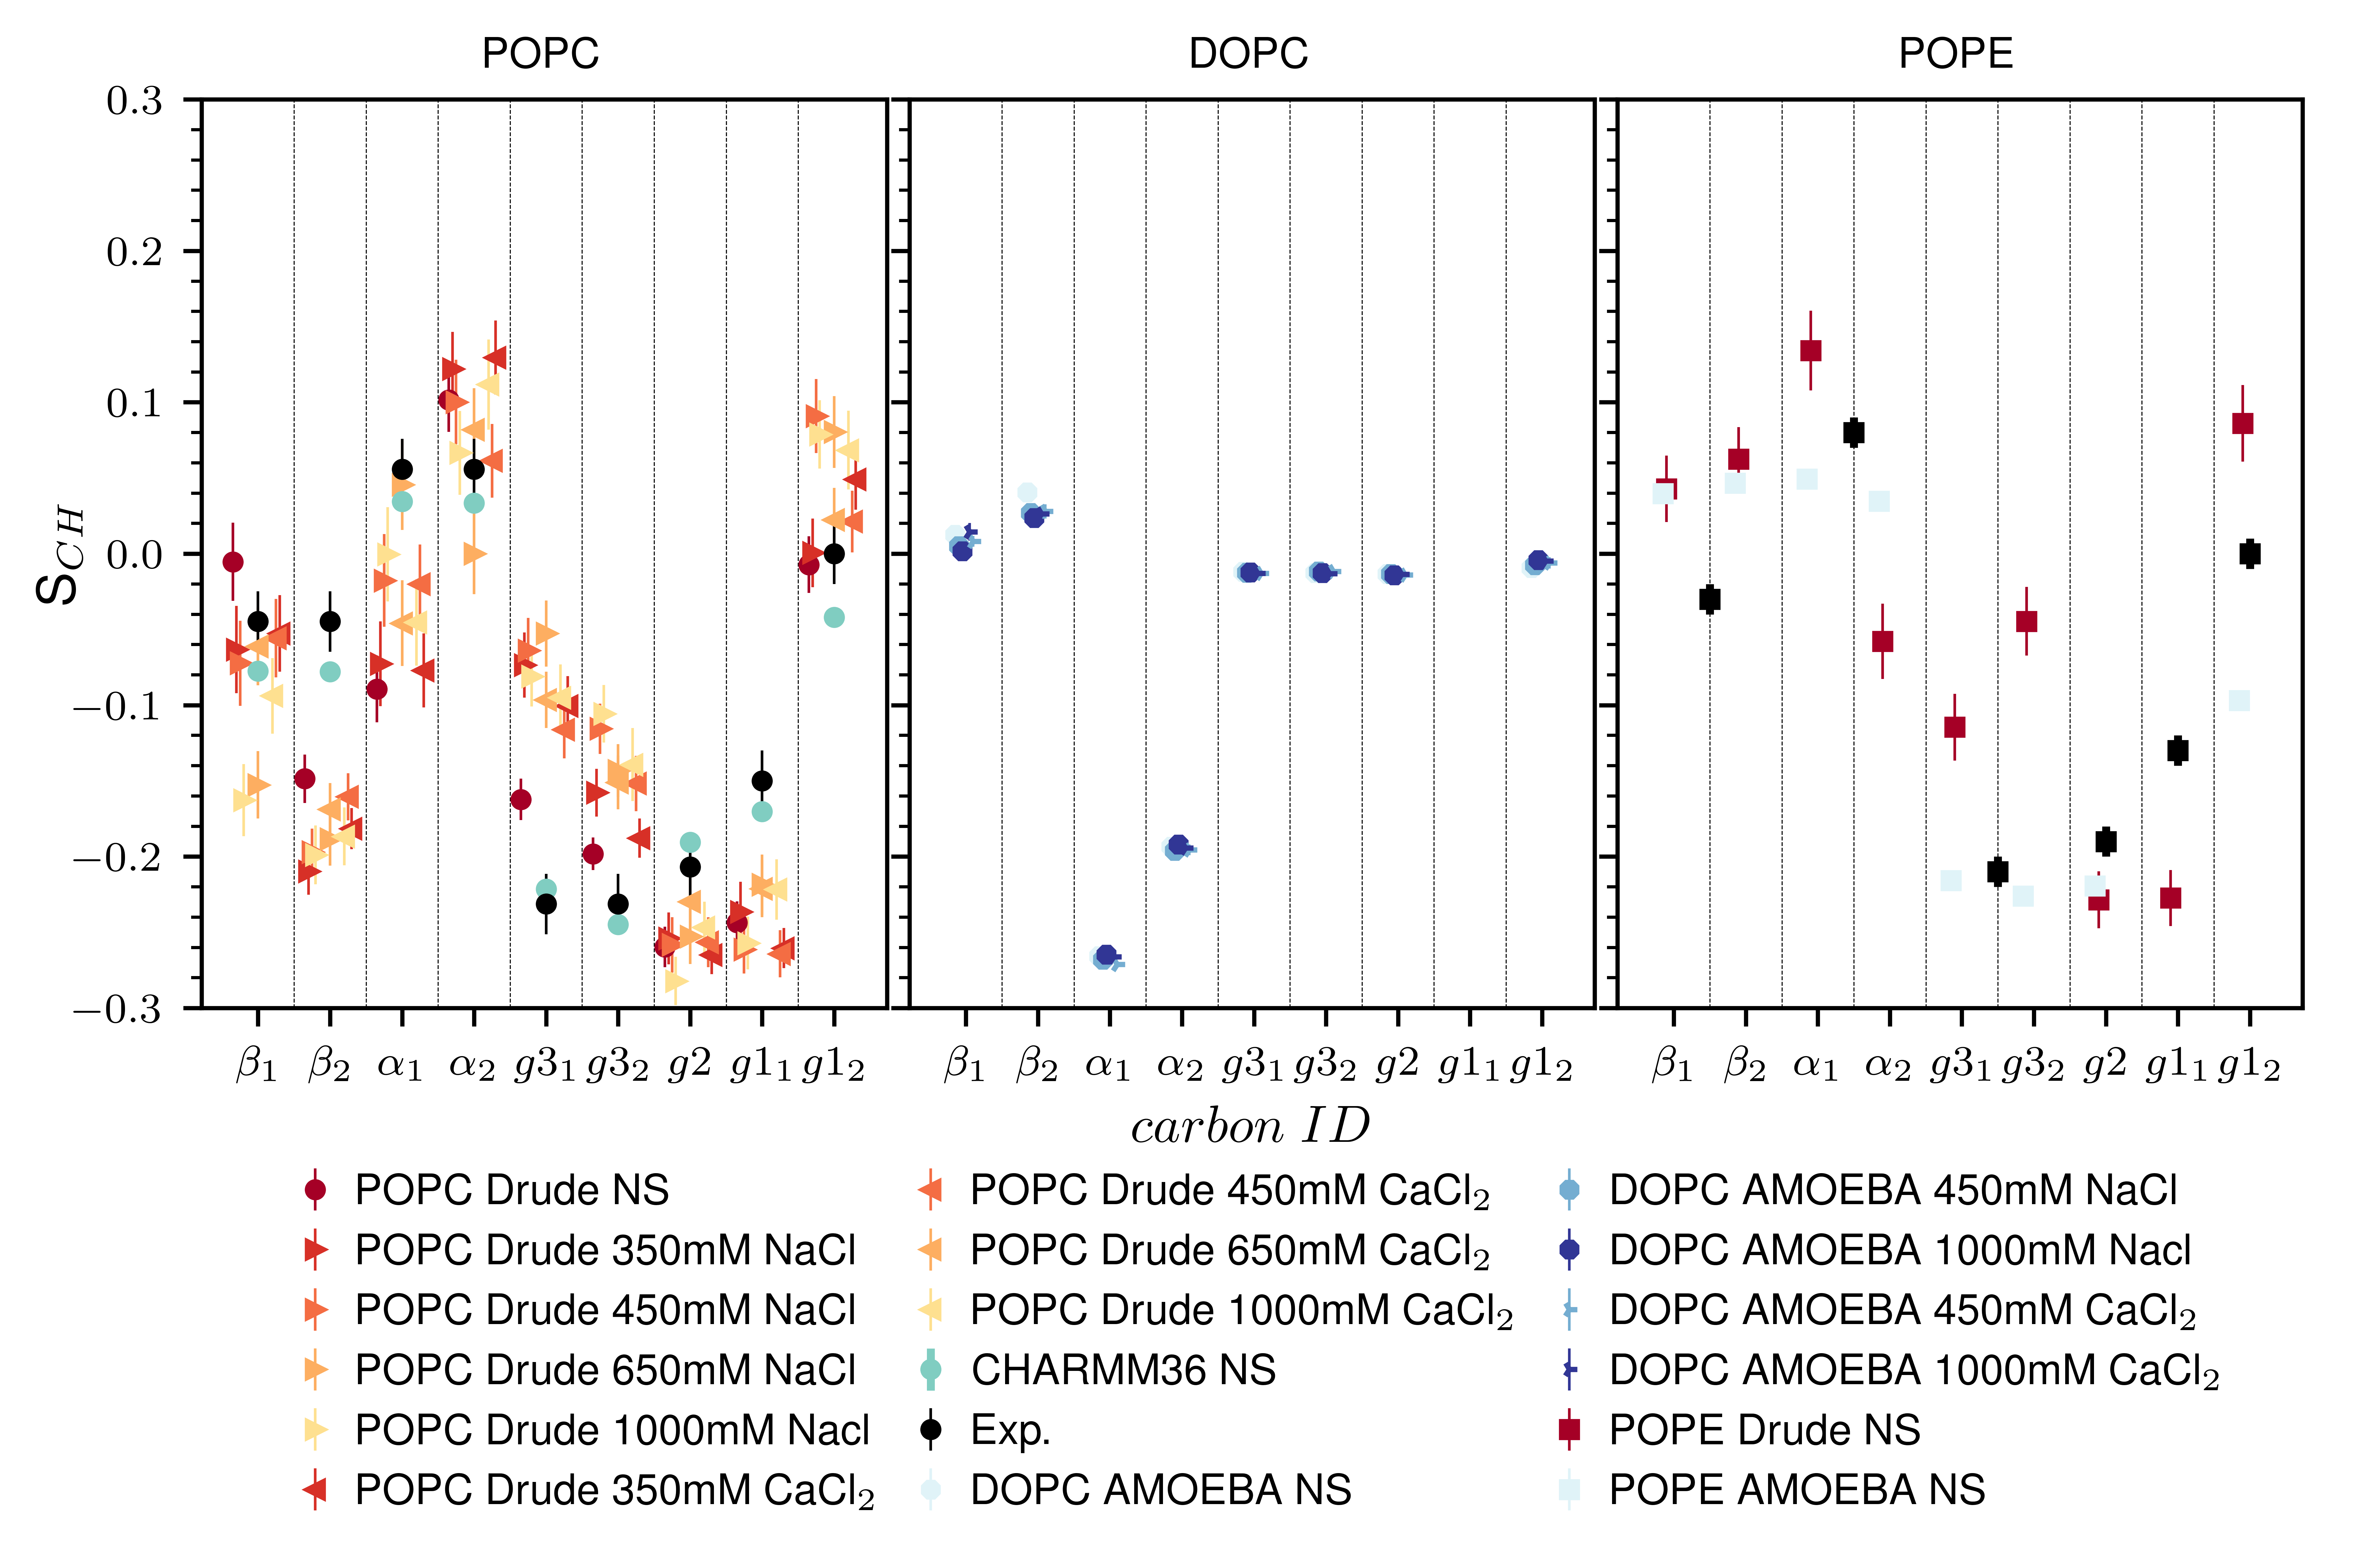
\includegraphics{Figures/order_parameters.png}
    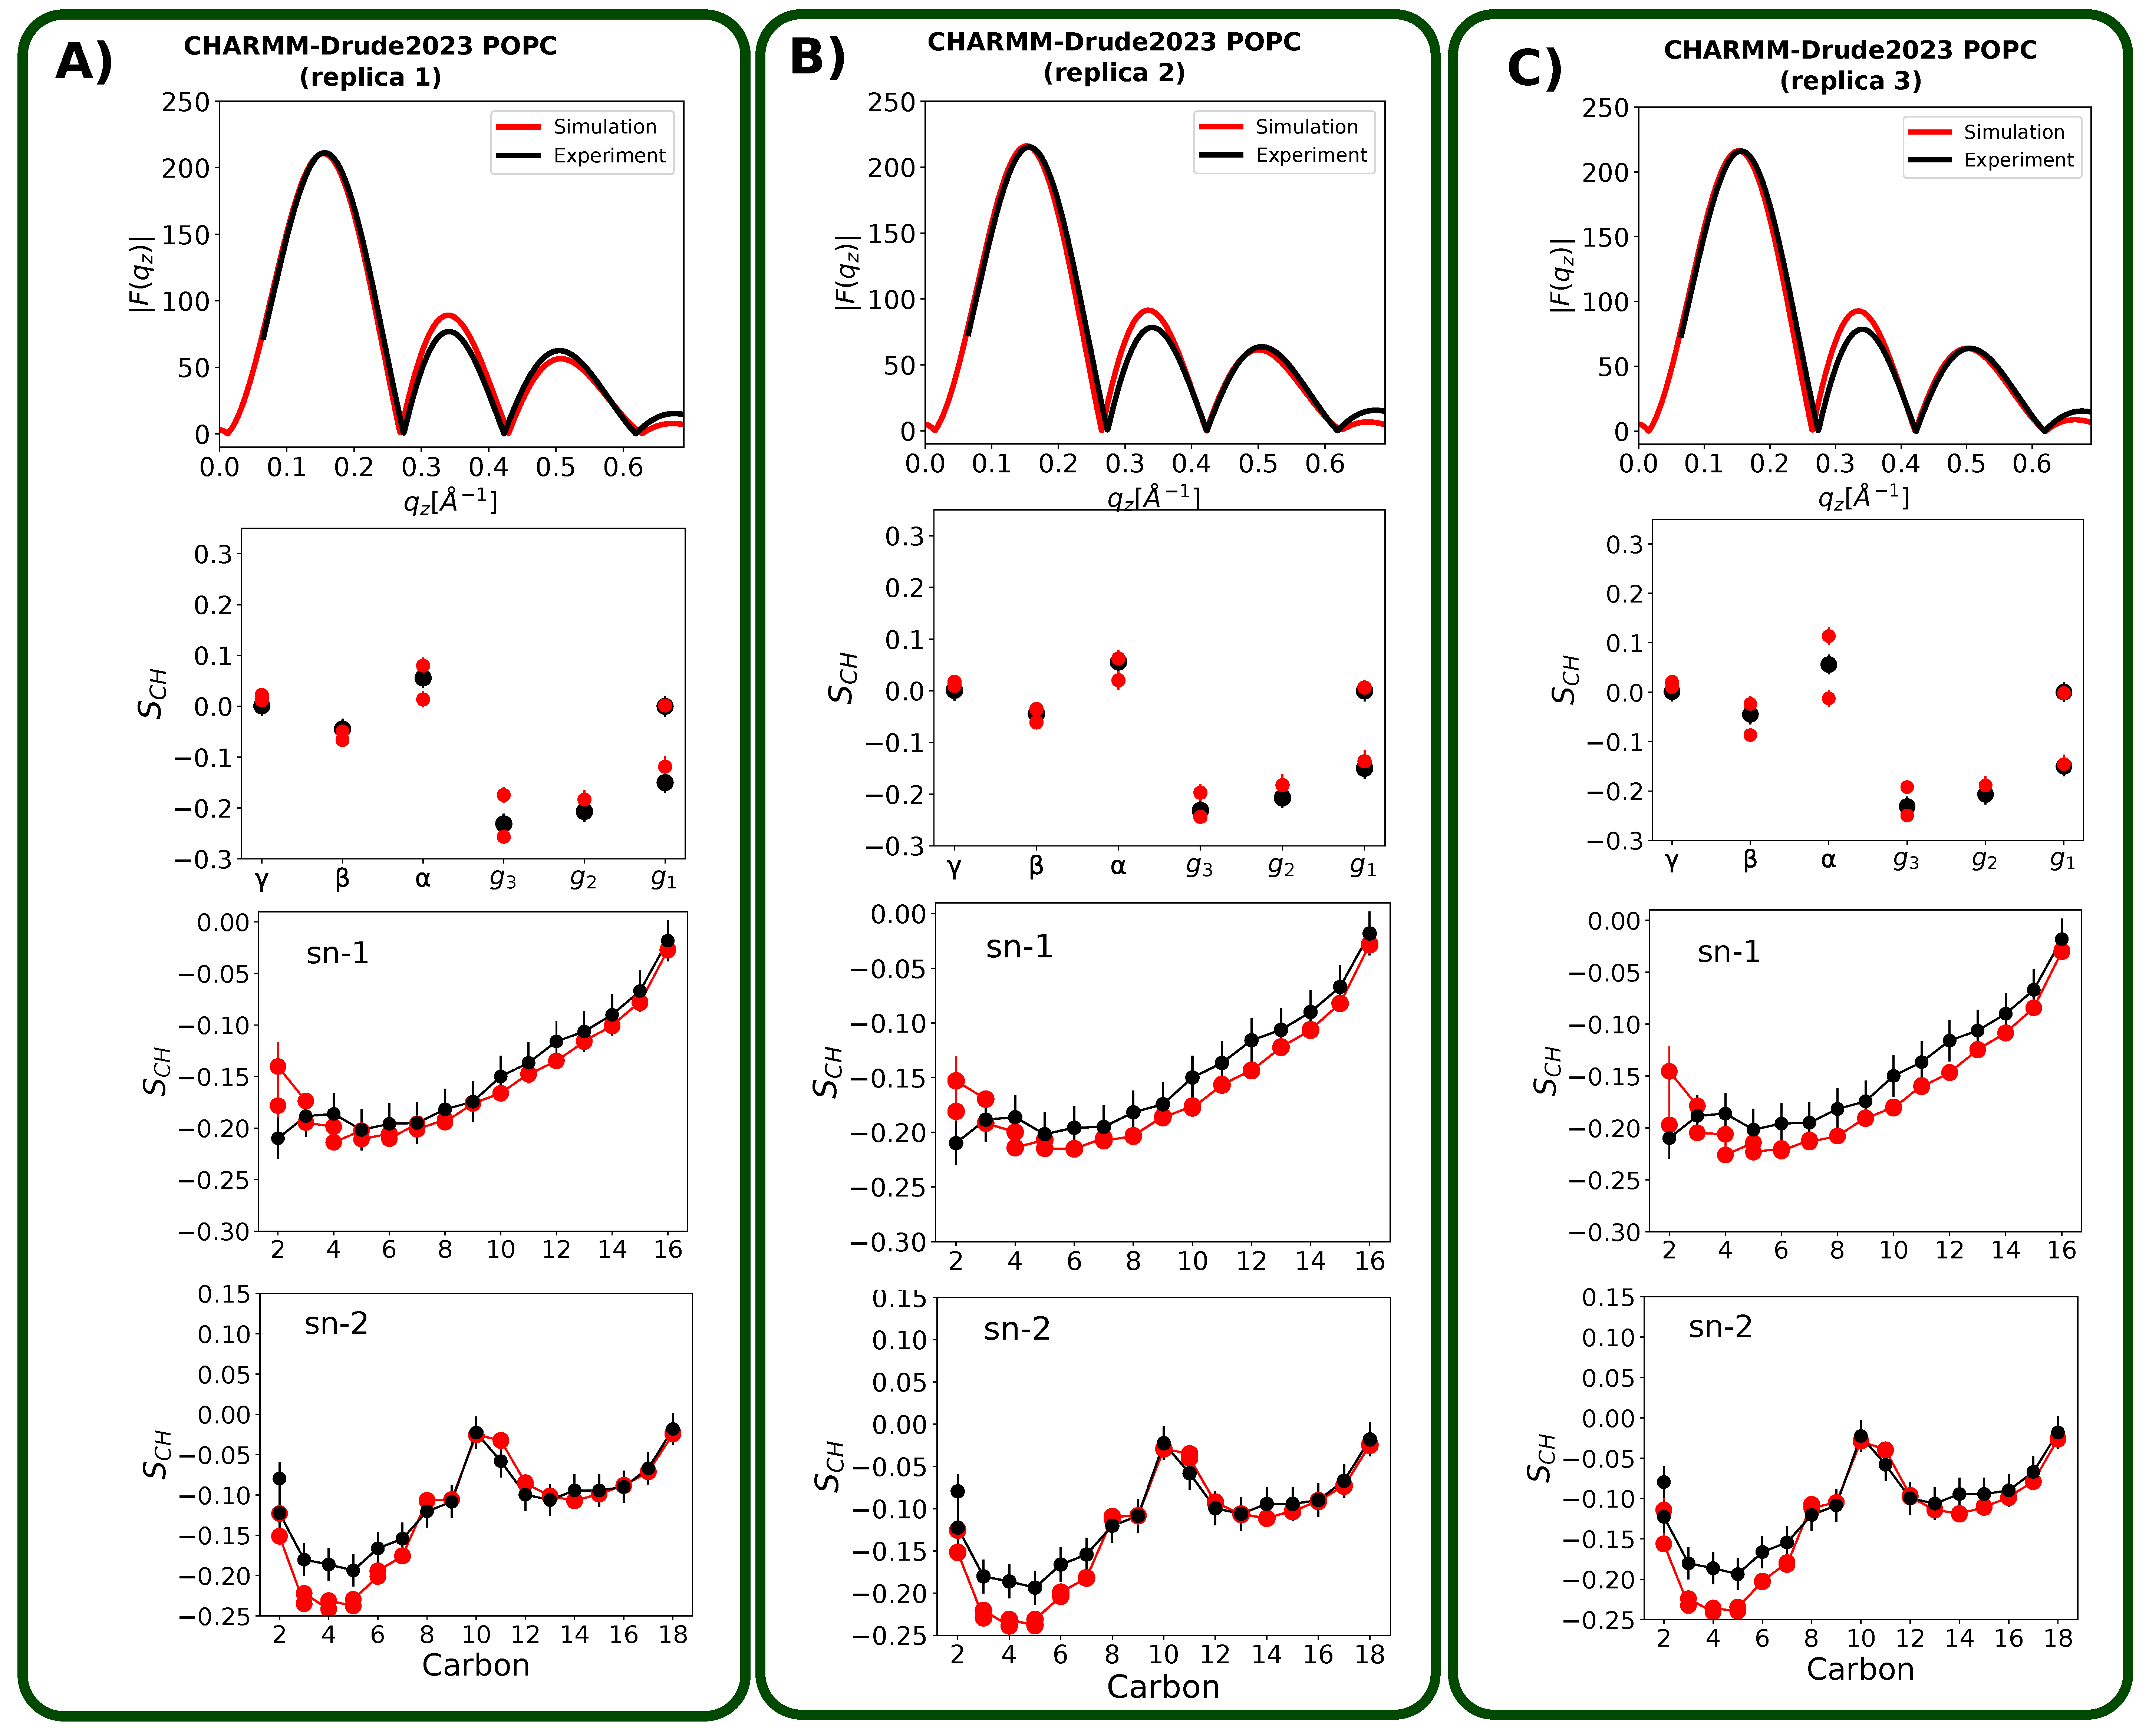
\includegraphics[width=0.8\textwidth]{Figures/quality_Drude2023_replicas.pdf}
    \caption{X-ray scattering form factors, and C-H bond order parameters for headgroup and glycerol backbone, and acyl chains (from top to bottom) compared between simulations and experiments using the NMRlipids databank. The atom labelling is as depicted in Fig.~\ref{fig:molecules}.}
    \label{fig:order_parameters_replicas}

\end{figure}

\begin{figure}[!hbt]
	\centering
	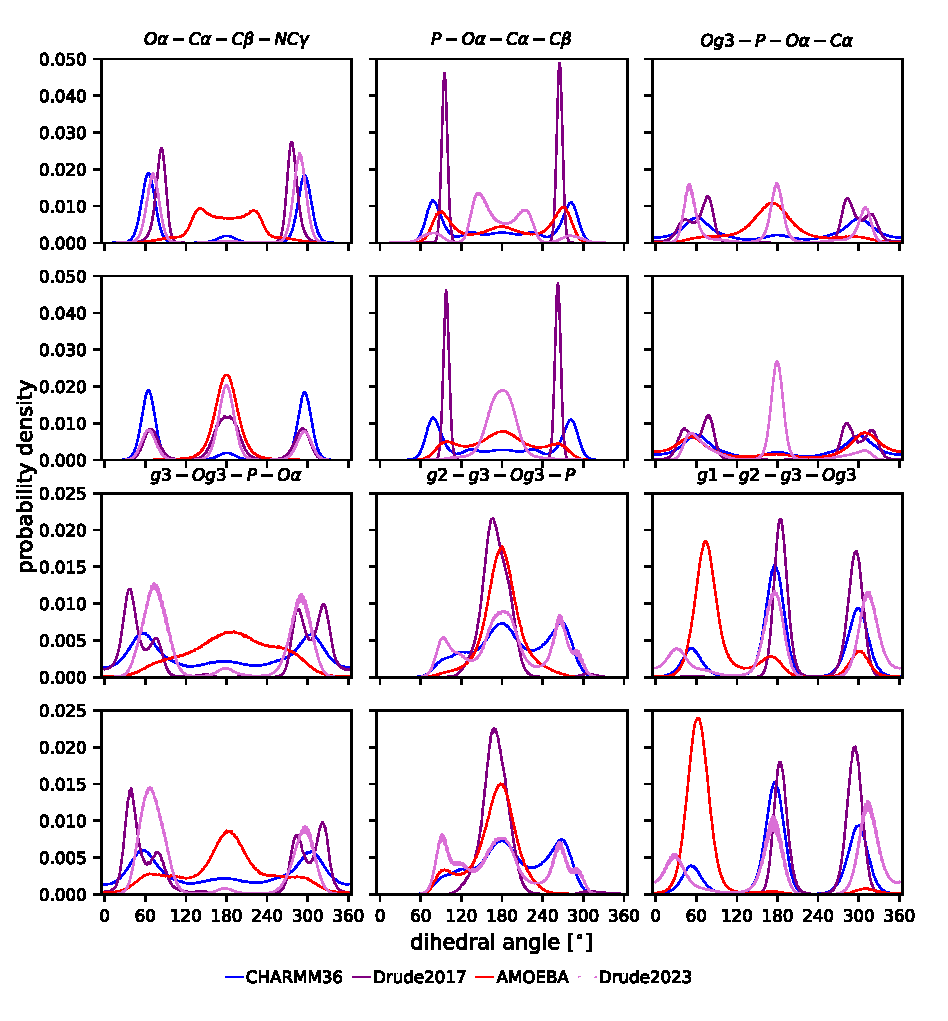
\includegraphics{Figures/dihedral_distributions_without_ions.eps}
	\caption{The distributions of the torsion angles for the head group atoms. For each torsion angle, the upper and lower rows contain the DOPC (AMOEBA) - POPC (Drude/Drude2023) and POPE lipids, respectively.}
	\label{fig:dihedral_no_salt}
\end{figure}



\end{document}
